\documentclass[11pt, letterpaper]{article}

% Fonts and Encoding
\usepackage[utf8]{inputenc}
\usepackage[T1]{fontenc}
\usepackage{lmodern} % High-quality Latin Modern vector font

% Math and Symbols
\usepackage{amsmath, amssymb, amsthm, amsfonts, mathrsfs, mathtools}

% Layout and Geometry
\usepackage{geometry}
\geometry{letterpaper, margin=1in}
\setlength{\parindent}{0pt}
\setlength{\parskip}{0.6em}

% Formatting and Graphics
\usepackage{graphicx, xcolor, enumitem, booktabs, array, tabularx}

% TikZ for Illustrations
\usepackage{tikz}
\usetikzlibrary{arrows.meta, positioning, shapes.geometric, calc, backgrounds, matrix}

% Clickable Links and TOC
\usepackage{hyperref}
\hypersetup{
    colorlinks=true,
    linkcolor=blue,
    filecolor=magenta,      
    urlcolor=cyan,
    pdftitle={Practice Problem Set: Inner Product, Length, and Orthogonality},
}

% Theorem Environments
\newtheorem{theorem}{Theorem}[section]
\newtheorem{lemma}[theorem]{Lemma}
\newtheorem{proposition}[theorem]{Proposition}
\newtheorem{corollary}[theorem]{Corollary}
\theoremstyle{definition}
\newtheorem{definition}{Definition}[section]
\newtheorem{axiom}{Axiom}[section]
\newtheorem{example}{Example}[section]
\theoremstyle{remark}
\newtheorem{remark}{Remark}[section]

% Custom Commands (Enforced standard notation)
\newcommand{\R}{\mathbb{R}}
\newcommand{\N}{\mathbb{N}}
\newcommand{\Z}{\mathbb{Z}}
\newcommand{\Q}{\mathbb{Q}}
\newcommand{\E}{\mathbb{E}}
\newcommand{\Prob}{\mathbb{P}}
\newcommand{\F}{\mathcal{F}}

\title{Practice Problem Set: Inner Product, Length, and Orthogonality}
\author{Tashfeen Omran}
\date{November 16, 2026}

\begin{document}

\maketitle
\tableofcontents
\newpage

\section{Concept Checklist and Question Mapping}

\begin{remark}
Only one section guide was provided in the source materials (\textit{Comprehensive Guide to Inner Product, Length, and Orthogonality}). Accordingly, this document presents a complete $30$-problem practice suite tailored to that section, placing heavier weight on advanced concepts (orthogonal projections, orthogonal complements and fundamental subspaces, the Cauchy-Schwarz inequality, algebraic proofs, diagnostic flaw analysis, and machine learning / quantitative finance modeling).
\end{remark}

Table~\ref{tab:concept-map-top} maps every core concept, algebraic technique, common pitfall, and extension from the section guide to the corresponding practice problems.

\begin{center}
\renewcommand{\arraystretch}{1.5}
\begin{tabularx}{\textwidth}{p{4.6cm} >{$\displaystyle}X<{$} l}
\toprule
\textbf{Concept / Problem Type} & \multicolumn{1}{l}{\textbf{Core Formula / Key Technique}} & \textbf{Problem(s)} \\
\midrule
Inner Product and Matrix Transpose Computation & \mathbf{u} \cdot \mathbf{v} = \mathbf{u}^T \mathbf{v} = \sum_{i=1}^{n} u_i v_i & 1, 2, 13, 30 \\
\addlinespace[4pt]
Vector Norm, Negative Squares, and Scalar Pull-Out & \|\mathbf{v}\| = \sqrt{\mathbf{v} \cdot \mathbf{v}},\quad \|c\mathbf{v}\| = |c|\|\mathbf{v}\| & 3, 4, 5, 27, 28 \\
\addlinespace[4pt]
Normalization, Unit Vectors, and Integer Scaling Trick & \hat{\mathbf{u}} = \frac{1}{\|\mathbf{v}\|}\mathbf{v}\quad (\text{clear denominators first}) & 5, 6, 28, 30 \\
\addlinespace[4pt]
Distance and Angle Between Vectors & \operatorname{dist}(\mathbf{u}, \mathbf{v}) = \|\mathbf{u} - \mathbf{v}\|,\quad \cos\theta = \frac{\mathbf{u}\cdot\mathbf{v}}{\|\mathbf{u}\|\|\mathbf{v}\|} & 7, 8, 9, 28, 29 \\
\addlinespace[4pt]
Orthogonality, Parameters, and Pythagorean Theorem & \mathbf{u} \perp \mathbf{v} \iff \mathbf{u}\cdot\mathbf{v} = 0 \iff \|\mathbf{u}+\mathbf{v}\|^2 = \|\mathbf{u}\|^2 + \|\mathbf{v}\|^2 & 10, 11, 12, 30 \\
\addlinespace[4pt]
Orthogonal Projection and Line Decomposition & \operatorname{proj}_{\mathbf{u}}\mathbf{y} = \left(\frac{\mathbf{y}\cdot\mathbf{u}}{\mathbf{u}\cdot\mathbf{u}}\right)\mathbf{u},\quad \mathbf{y} = \hat{\mathbf{y}} + \mathbf{z}\ (\mathbf{z} \perp \mathbf{u}) & 13, 14, 15, 16, 26, 30 \\
\addlinespace[4pt]
Orthogonal Complements and Fundamental Subspaces & W^{\perp\vphantom{A}},\quad \operatorname{Row}(A)^{\perp\vphantom{A}} = \operatorname{Nul}(A),\quad \operatorname{Col}(A)^{\perp\vphantom{A}} = \operatorname{Nul}(A^T) & 17, 18, 19, 25, 27, 30 \\
\addlinespace[4pt]
Cauchy-Schwarz and Triangle Inequalities & |\mathbf{u}\cdot\mathbf{v}| \le \|\mathbf{u}\|\|\mathbf{v}\|,\quad \|\mathbf{u}+\mathbf{v}\| \le \|\mathbf{u}\| + \|\mathbf{v}\| & 20, 21, 22 \\
\addlinespace[4pt]
Algebraic Proofs and Geometric Vector Identities & \|\mathbf{u}+\mathbf{v}\|^2 + \|\mathbf{u}-\mathbf{v}\|^2 = 2\|\mathbf{u}\|^2 + 2\|\mathbf{v}\|^2 & 23, 24, 25, 26 \\
\addlinespace[4pt]
Conceptual Diagnostics and ``Find the Flaw'' Traps & (\mathbf{u}\cdot\mathbf{v})\mathbf{w}\ \text{vs.\ invalid}\ (\mathbf{u}\cdot\mathbf{v})\cdot\mathbf{w},\ \text{missing}\ \sqrt{\cdot} & 4, 7, 27, 28 \\
\addlinespace[4pt]
Real-World Modeling (SVM Margin and Quant Finance) & d_i = \frac{|\mathbf{w}\cdot\mathbf{x}_i + b|}{\|\mathbf{w}\|},\quad \text{margin} = \frac{2}{\|\mathbf{w}\|},\quad \text{PCA factors} & 29, 30 \\
\bottomrule
\end{tabularx}
\captionof{table}{Concept checklist and problem mapping for Inner Product, Length, and Orthogonality.}
\label{tab:concept-map-top}
\end{center}

\newpage
\section{Problem Sets}

\subsection{Foundational Computations, Norms, and Normalization}

\textbf{Problem 1:} Let $\mathbf{u} = \begin{bmatrix} 3 \\ -2 \end{bmatrix}$ and $\mathbf{v} = \begin{bmatrix} -4 \\ 5 \end{bmatrix}$ in $\mathbb{R}^2$. Compute each of the following expressions:
\begin{enumerate}[label=(\alph*)]
    \item $\mathbf{u} \cdot \mathbf{u}$
    \item $\mathbf{v}^T \mathbf{u}$
    \item $\frac{\mathbf{u} \cdot \mathbf{v}}{\mathbf{u} \cdot \mathbf{u}}$
    \item $\left(\frac{\mathbf{u} \cdot \mathbf{v}}{\mathbf{v} \cdot \mathbf{v}}\right)\mathbf{v}$
\end{enumerate}

\textbf{Problem 2:} Let $\mathbf{a} = \begin{bmatrix} 2 \\ -1 \\ 4 \\ 0 \end{bmatrix}$, $\mathbf{b} = \begin{bmatrix} -3 \\ 5 \\ 1 \\ -2 \end{bmatrix}$, and $\mathbf{c} = \begin{bmatrix} 1 \\ 2 \\ -1 \\ 3 \end{bmatrix}$ in $\mathbb{R}^4$. Compute:
\begin{enumerate}[label=(\alph*)]
    \item $\mathbf{a} \cdot \mathbf{b}$
    \item $(2\mathbf{a} - \mathbf{c}) \cdot \mathbf{b}$ using the linearity properties of the inner product, and verify your result by first computing $2\mathbf{a} - \mathbf{c}$ directly.
    \item $\mathbf{b}^T \mathbf{b} - (\mathbf{a} \cdot \mathbf{c})^2$
\end{enumerate}

\textbf{Problem 3:} Compute the length (norm) $\|\mathbf{v}\|$ of each vector by first factoring out the greatest common divisor (the Scalar Pull-Out trick):
\begin{enumerate}[label=(\alph*)]
    \item $\mathbf{v}_1 = \begin{bmatrix} -45 \\ 60 \end{bmatrix}$
    \item $\mathbf{v}_2 = \begin{bmatrix} 14 \\ -28 \\ 28 \end{bmatrix}$
\end{enumerate}

\textbf{Problem 4:} Let $\mathbf{w} = \begin{bmatrix} -2 \\ 1 \\ -2 \\ 4 \end{bmatrix} \in \mathbb{R}^4$ and let $c = -3$.
\begin{enumerate}[label=(\alph*)]
    \item Compute $\|\mathbf{w}\|$ directly, taking care with negative entries.
    \item Compute $\|c\mathbf{w}\|$ using the norm scaling identity $\|c\mathbf{w}\| = |c|\|\mathbf{w}\|$, and briefly explain why writing $\|c\mathbf{w}\| = c\|\mathbf{w}\|$ would be mathematically incorrect here.
    \item Find all real numbers $k$ such that $\|k\mathbf{w}\| = 15$.
\end{enumerate}

\textbf{Problem 5:} Consider the vector $\mathbf{p} = \begin{bmatrix} -24 \\ 70 \end{bmatrix} \in \mathbb{R}^2$.
\begin{enumerate}[label=(\alph*)]
    \item Find the unit vector $\hat{\mathbf{p}}$ in the direction of $\mathbf{p}$ using the Scalar Pull-Out trick.
    \item Find a vector $\mathbf{q}$ of length $10$ pointing in the direction \emph{opposite} to $\mathbf{p}$.
\end{enumerate}

\textbf{Problem 6:} Find a unit vector $\hat{\mathbf{u}}$ in the direction of $\mathbf{v} = \begin{bmatrix} 3/8 \\ -1/4 \\ 1/2 \\ -1 \end{bmatrix} \in \mathbb{R}^4$ by first clearing fractions via the Integer Scaling Trick. Verify explicitly that $\|\hat{\mathbf{u}}\| = 1$.

\subsection{Distance, Angles, and Orthogonality Conditions}

\textbf{Problem 7:} Find the distance $\operatorname{dist}(\mathbf{x}, \mathbf{y})$ between $\mathbf{x} = \begin{bmatrix} 4 \\ -7 \\ 2 \end{bmatrix}$ and $\mathbf{y} = \begin{bmatrix} -2 \\ -4 \\ 8 \end{bmatrix}$, and verify explicitly that $|\|\mathbf{x}\| - \|\mathbf{y}\|| \neq \operatorname{dist}(\mathbf{x}, \mathbf{y})$.

\textbf{Problem 8:} Find all real values of $t$ such that the distance between $\mathbf{u} = \begin{bmatrix} t \\ -1 \\ 3 \end{bmatrix}$ and $\mathbf{v} = \begin{bmatrix} 2 \\ t \\ -1 \end{bmatrix}$ is $3\sqrt{5}$.

\textbf{Problem 9:} For each pair of vectors below, compute $\cos\theta$, find the exact angle $\theta \in [0, \pi]$ in radians between the vectors, and classify the angle as acute, right, or obtuse:
\begin{enumerate}[label=(\alph*)]
    \item $\mathbf{u} = \begin{bmatrix} 1 \\ -1 \\ 0 \end{bmatrix}$ and $\mathbf{v} = \begin{bmatrix} 0 \\ 1 \\ -1 \end{bmatrix}$ in $\mathbb{R}^3$.
    \item $\mathbf{a} = \begin{bmatrix} 1 \\ 1 \\ 1 \\ 1 \end{bmatrix}$ and $\mathbf{b} = \begin{bmatrix} 1 \\ 1 \\ 0 \\ 0 \end{bmatrix}$ in $\mathbb{R}^4$.
\end{enumerate}

\textbf{Problem 10:} Determine whether each pair of vectors is orthogonal:
\begin{enumerate}[label=(\alph*)]
    \item $\mathbf{u} = \begin{bmatrix} 6 \\ -4 \\ 2 \end{bmatrix}$ and $\mathbf{v} = \begin{bmatrix} 3 \\ 5 \\ 1 \end{bmatrix}$
    \item $\mathbf{p} = \begin{bmatrix} 5 \\ -3 \\ 2 \\ -1 \end{bmatrix}$ and $\mathbf{q} = \begin{bmatrix} 2 \\ 4 \\ 3 \\ 5 \end{bmatrix}$
\end{enumerate}

\textbf{Problem 11:}
\begin{enumerate}[label=(\alph*)]
    \item Find all real values of $k$ such that $\mathbf{u} = \begin{bmatrix} k \\ k \\ -3 \end{bmatrix}$ and $\mathbf{v} = \begin{bmatrix} k \\ -2 \\ 1 \end{bmatrix}$ are orthogonal.
    \item Find a nonzero vector $\mathbf{w} \in \mathbb{R}^3$ that is simultaneously orthogonal to both $\mathbf{a} = \begin{bmatrix} 1 \\ -2 \\ 1 \end{bmatrix}$ and $\mathbf{b} = \begin{bmatrix} 2 \\ 1 \\ -3 \end{bmatrix}$.
\end{enumerate}

\textbf{Problem 12:}
\begin{enumerate}[label=(\alph*)]
    \item Let $\mathbf{u} = \begin{bmatrix} 2 \\ -1 \\ 2 \\ 0 \end{bmatrix}$ and $\mathbf{v} = \begin{bmatrix} 1 \\ 4 \\ 1 \\ -2 \end{bmatrix}$ in $\mathbb{R}^4$. Verify that $\mathbf{u}$ and $\mathbf{v}$ satisfy the Pythagorean identity $\|\mathbf{u} + \mathbf{v}\|^2 = \|\mathbf{u}\|^2 + \|\mathbf{v}\|^2$.
    \item Consider the triangle in $\mathbb{R}^3$ with vertices $O = \mathbf{0}$, $P = \mathbf{p} = \begin{bmatrix} 2 \\ 1 \\ -1 \end{bmatrix}$, and $Q = \mathbf{q} = \begin{bmatrix} 3 \\ 3 \\ 3 \end{bmatrix}$. Determine whether $\triangle OPQ$ is a right triangle, and if so, identify which vertex has the right angle.
\end{enumerate}

\subsection{Orthogonal Projections and Decomposition}

\textbf{Problem 13:} Let $\mathbf{y} = \begin{bmatrix} 7 \\ 6 \end{bmatrix}$ and $\mathbf{u} = \begin{bmatrix} 4 \\ 2 \end{bmatrix}$ in $\mathbb{R}^2$.
\begin{enumerate}[label=(\alph*)]
    \item Compute the orthogonal projection $\hat{\mathbf{y}} = \operatorname{proj}_{\mathbf{u}}\mathbf{y} = \left(\frac{\mathbf{y}\cdot\mathbf{u}}{\mathbf{u}\cdot\mathbf{u}}\right)\mathbf{u}$.
    \item Compute the orthogonal component $\mathbf{z} = \mathbf{y} - \hat{\mathbf{y}}$ and verify explicitly that $\mathbf{z} \perp \mathbf{u}$.
    \item Verify that $\|\mathbf{y}\|^2 = \|\hat{\mathbf{y}}\|^2 + \|\mathbf{z}\|^2$.
\end{enumerate}

\textbf{Problem 14:} Let $\mathbf{y} = \begin{bmatrix} 1 \\ 3 \\ 5 \end{bmatrix}$ and let $L = \operatorname{Span}\{\mathbf{u}\} \subset \mathbb{R}^3$, where $\mathbf{u} = \begin{bmatrix} 1 \\ -1 \\ 2 \end{bmatrix}$.
\begin{enumerate}[label=(\alph*)]
    \item Decompose $\mathbf{y}$ as $\mathbf{y} = \hat{\mathbf{y}} + \mathbf{z}$, where $\hat{\mathbf{y}} \in L$ and $\mathbf{z} \perp L$.
    \item Determine the shortest distance from the point $\mathbf{y}$ to the line $L$.
\end{enumerate}

\textbf{Problem 15:} Let $\mathbf{u}, \mathbf{y} \in \mathbb{R}^n$ with $\mathbf{u} \neq \mathbf{0}$.
\begin{enumerate}[label=(\alph*)]
    \item Prove that for any nonzero scalar $c \in \mathbb{R} \setminus \{0\}$, $\operatorname{proj}_{c\mathbf{u}}\mathbf{y} = \operatorname{proj}_{\mathbf{u}}\mathbf{y}$.
    \item Prove that $\operatorname{proj}_{\mathbf{u}}(\operatorname{proj}_{\mathbf{u}}\mathbf{y}) = \operatorname{proj}_{\mathbf{u}}\mathbf{y}$ (idempotence).
    \item Use part (a) to compute $\operatorname{proj}_{\mathbf{u}}\mathbf{y}$ efficiently when $\mathbf{u} = \begin{bmatrix} 1/5 \\ -2/5 \\ 2/5 \end{bmatrix}$ and $\mathbf{y} = \begin{bmatrix} 4 \\ 1 \\ 8 \end{bmatrix}$.
\end{enumerate}

\textbf{Problem 16:} Let $\mathbf{u} = \begin{bmatrix} 2 \\ -1 \\ 2 \end{bmatrix}$ and $\mathbf{y} = \begin{bmatrix} a \\ 4 \\ b \end{bmatrix}$ in $\mathbb{R}^3$. Suppose that $\operatorname{proj}_{\mathbf{u}}\mathbf{y} = \begin{bmatrix} 4 \\ -2 \\ 4 \end{bmatrix}$ and $\|\mathbf{y}\|^2 = 77$.
\begin{enumerate}[label=(\alph*)]
    \item Find the linear equation relating $a$ and $b$ implied by the given projection.
    \item Determine all possible vectors $\mathbf{y}$ satisfying both conditions.
\end{enumerate}

\subsection{Orthogonal Complements and Fundamental Subspaces}

\textbf{Problem 17:} Let $W = \operatorname{Span}\{\mathbf{v}_1, \mathbf{v}_2\} \subset \mathbb{R}^4$, where $\mathbf{v}_1 = \begin{bmatrix} 1 \\ -2 \\ 3 \\ 1 \end{bmatrix}$ and $\mathbf{v}_2 = \begin{bmatrix} 2 \\ 1 \\ 0 \\ -1 \end{bmatrix}$.
\begin{enumerate}[label=(\alph*)]
    \item Determine whether $\mathbf{x} = \begin{bmatrix} 1 \\ 1 \\ 1 \\ -2 \end{bmatrix}$ lies in $W^{\perp}$.
    \item Determine whether $\mathbf{z} = \begin{bmatrix} 1 \\ 0 \\ -1 \\ 2 \end{bmatrix}$ lies in $W^{\perp}$.
    \item Explain briefly why checking $\mathbf{z} \cdot \mathbf{v}_1 = 0$ and $\mathbf{z} \cdot \mathbf{v}_2 = 0$ is sufficient to guarantee that $\mathbf{z}$ is orthogonal to \emph{every} vector in $W$.
\end{enumerate}

\textbf{Problem 18:} Let $W = \operatorname{Span}\left\{\begin{bmatrix} 1 \\ 2 \\ -1 \\ 3 \end{bmatrix}, \begin{bmatrix} 2 \\ 5 \\ 0 \\ 4 \end{bmatrix}\right\} \subset \mathbb{R}^4$.
\begin{enumerate}[label=(\alph*)]
    \item Construct a matrix $A$ such that $W = \operatorname{Row}(A)$, and explain why $W^{\perp} = \operatorname{Nul}(A)$.
    \item Find a basis for $W^{\perp}$.
    \item Verify directly that each basis vector you found for $W^{\perp}$ is orthogonal to both spanning vectors of $W$.
\end{enumerate}

\textbf{Problem 19:} Let $A = \begin{bmatrix} 1 & -2 \\ 2 & -3 \\ -1 & 1 \end{bmatrix}$.
\begin{enumerate}[label=(\alph*)]
    \item Prove in general that for any $m \times n$ matrix $M$, $(\operatorname{Col} M)^{\perp} = \operatorname{Nul}(M^T)$.
    \item Find a basis for $(\operatorname{Col} A)^{\perp}$.
    \item Verify whether $\mathbf{b} = \begin{bmatrix} -2 \\ 2 \\ 2 \end{bmatrix}$ belongs to $(\operatorname{Col} A)^{\perp}$, and explain what this implies about the consistency of the linear system $A\mathbf{x} = \mathbf{b}$.
\end{enumerate}

\subsection{Cauchy-Schwarz and Triangle Inequalities}

\textbf{Problem 20:}
\begin{enumerate}[label=(\alph*)]
    \item Verify the Cauchy-Schwarz Inequality $|\mathbf{u} \cdot \mathbf{v}| \le \|\mathbf{u}\|\|\mathbf{v}\|$ for $\mathbf{u} = \begin{bmatrix} 2 \\ -3 \\ 6 \end{bmatrix}$ and $\mathbf{v} = \begin{bmatrix} -4 \\ 1 \\ 2 \end{bmatrix}$.
    \item For $\mathbf{p} = \begin{bmatrix} 3 \\ -4 \end{bmatrix}$ and $\mathbf{q} = \begin{bmatrix} -6 \\ 8 \end{bmatrix}$, show that equality holds in the Cauchy-Schwarz Inequality, and state the general condition on $\mathbf{u}$ and $\mathbf{v}$ under which $|\mathbf{u} \cdot \mathbf{v}| = \|\mathbf{u}\|\|\mathbf{v}\|$.
\end{enumerate}

\textbf{Problem 21:} Suppose $\mathbf{u}, \mathbf{v} \in \mathbb{R}^5$ satisfy $\|\mathbf{u}\| = 4$ and $\|\mathbf{v}\| = 7$.
\begin{enumerate}[label=(\alph*)]
    \item Find the exact minimum and maximum possible values of $\mathbf{u} \cdot \mathbf{v}$.
    \item Find the exact minimum and maximum possible values of $\|\mathbf{u} + \mathbf{v}\|$ and $\|\mathbf{u} - \mathbf{v}\|$.
    \item Describe the geometric orientation of $\mathbf{u}$ and $\mathbf{v}$ when $\|\mathbf{u} - \mathbf{v}\|$ achieves its maximum value.
\end{enumerate}

\textbf{Problem 22:}
\begin{enumerate}[label=(\alph*)]
    \item Assuming the Cauchy-Schwarz Inequality $|\mathbf{u} \cdot \mathbf{v}| \le \|\mathbf{u}\|\|\mathbf{v}\|$, prove the Triangle Inequality for all $\mathbf{u}, \mathbf{v} \in \mathbb{R}^n$:
    \[
    \|\mathbf{u} + \mathbf{v}\| \le \|\mathbf{u}\| + \|\mathbf{v}\|
    \]
    \item By applying the Cauchy-Schwarz Inequality to an appropriately chosen pair of vectors in $\mathbb{R}^n$, prove that for all real numbers $x_1, x_2, \dots, x_n$:
    \[
    \left(\sum_{i=1}^{n} x_i\right)^2 \le n \sum_{i=1}^{n} x_i^2
    \]
\end{enumerate}

\subsection{Algebraic Proofs and Geometric Identities}

\textbf{Problem 23:}
\begin{enumerate}[label=(\alph*)]
    \item For any vectors $\mathbf{u}, \mathbf{v} \in \mathbb{R}^n$, prove the Polarization Identity:
    \[
    \mathbf{u} \cdot \mathbf{v} = \frac{1}{4}\left(\|\mathbf{u} + \mathbf{v}\|^2 - \|\mathbf{u} - \mathbf{v}\|^2\right)
    \]
    \item Suppose $\mathbf{u}, \mathbf{v} \in \mathbb{R}^n$ satisfy $\|\mathbf{u} + \mathbf{v}\| = 9$ and $\|\mathbf{u} - \mathbf{v}\| = 5$. Use part (a) to compute $\mathbf{u} \cdot \mathbf{v}$.
\end{enumerate}

\textbf{Problem 24:}
\begin{enumerate}[label=(\alph*)]
    \item For any vectors $\mathbf{u}, \mathbf{v} \in \mathbb{R}^n$ and any scalars $a, b \in \mathbb{R}$, prove the generalized identity:
    \[
    \|a\mathbf{u} + b\mathbf{v}\|^2 + \|b\mathbf{u} - a\mathbf{v}\|^2 = (a^2 + b^2)\left(\|\mathbf{u}\|^2 + \|\mathbf{v}\|^2\right)
    \]
    Explain briefly how setting $a = b = 1$ yields the Parallelogram Law.
    \item Prove that $\|\mathbf{u} + \mathbf{v}\| = \|\mathbf{u} - \mathbf{v}\|$ if and only if $\mathbf{u} \perp \mathbf{v}$ (a parallelogram has diagonals of equal length if and only if it is a rectangle).
\end{enumerate}

\textbf{Problem 25:} Let $W$ be any nonempty subset of $\mathbb{R}^n$, and define $W^{\perp} = \{\mathbf{x} \in \mathbb{R}^n \mid \mathbf{x} \cdot \mathbf{w} = 0 \text{ for all } \mathbf{w} \in W\}$.
\begin{enumerate}[label=(\alph*)]
    \item Suppose a vector $\mathbf{y} \in \mathbb{R}^n$ is orthogonal to vectors $\mathbf{u}$ and $\mathbf{v}$. Show that $\mathbf{y}$ is orthogonal to any linear combination $c_1\mathbf{u} + c_2\mathbf{v}$, where $c_1, c_2 \in \mathbb{R}$.
    \item Prove rigorously that $W^{\perp}$ is a subspace of $\mathbb{R}^n$ by verifying the three subspace axioms.
\end{enumerate}

\textbf{Problem 26:}
\begin{enumerate}[label=(\alph*)]
    \item Prove that for any $\mathbf{u}, \mathbf{v} \in \mathbb{R}^n$, $\|\mathbf{u}\| = \|\mathbf{v}\|$ if and only if $(\mathbf{u} + \mathbf{v}) \perp (\mathbf{u} - \mathbf{v})$ (geometrically, the diagonals of a parallelogram are perpendicular if and only if the parallelogram is a rhombus).
    \item Suppose $\mathbf{u}, \mathbf{v} \in \mathbb{R}^n$ satisfy $\mathbf{u} \cdot \mathbf{v} = \|\mathbf{u}\|^2$. Prove that $\mathbf{u}$ is orthogonal to $\mathbf{v} - \mathbf{u}$, and interpret this geometrically when $\mathbf{u} \neq \mathbf{0}$.
\end{enumerate}

\subsection{Conceptual Diagnostics and Pitfall Analysis}

\textbf{Problem 27:} Determine whether each statement is \textbf{True} or \textbf{False}. Provide a brief proof if the statement is true, or a concrete counterexample in $\mathbb{R}^2$ (or explanation) if it is false.
\begin{enumerate}[label=(\alph*)]
    \item For every vector $\mathbf{v} \in \mathbb{R}^n$ and every scalar $c \in \mathbb{R}$, $\|c\mathbf{v}\| = c\|\mathbf{v}\|$.
    \item If $\mathbf{u}, \mathbf{v}, \mathbf{w} \in \mathbb{R}^n$ satisfy $\mathbf{u} \cdot \mathbf{v} = \mathbf{u} \cdot \mathbf{w}$ and $\mathbf{u} \neq \mathbf{0}$, then $\mathbf{v} = \mathbf{w}$.
    \item The zero vector $\mathbf{0} \in \mathbb{R}^n$ is the unique vector belonging to both a subspace $W$ and its orthogonal complement $W^{\perp}$.
    \item For all $\mathbf{u}, \mathbf{v} \in \mathbb{R}^n$, $\|\mathbf{u} - \mathbf{v}\|^2 = \|\mathbf{u}\|^2 - \|\mathbf{v}\|^2$.
    \item For any $\mathbf{u}, \mathbf{v}, \mathbf{w} \in \mathbb{R}^n$, the expression $(\mathbf{u} \cdot \mathbf{v}) \cdot \mathbf{w}$ is always a well-defined scalar.
    \item If vectors $\mathbf{v}_1, \dots, \mathbf{v}_p$ span a subspace $W \subset \mathbb{R}^n$ and $\mathbf{x} \in \mathbb{R}^n$ is orthogonal to each $\mathbf{v}_j$ ($j = 1, \dots, p$), then $\mathbf{x} \in W^{\perp}$.
\end{enumerate}

\textbf{Problem 28 (Find the Flaw):} Each of the following worked solutions contains a single critical error. Identify the flaw, explain why it is invalid in one sentence, and provide the correct final answer.
\begin{enumerate}[label=(\alph*)]
    \item \textit{Task:} Find the length of $\mathbf{v} = \begin{bmatrix} -5 \\ 12 \end{bmatrix}$. \\
    \textit{Flawed Solution:} $\|\mathbf{v}\| = \sqrt{(-5)^2 + 12^2} = \sqrt{-25 + 144} = \sqrt{119}$.
    \item \textit{Task:} Find the distance between $\mathbf{u} = \begin{bmatrix} 5 \\ 0 \end{bmatrix}$ and $\mathbf{v} = \begin{bmatrix} 0 \\ 12 \end{bmatrix}$. \\
    \textit{Flawed Solution:} $\|\mathbf{u}\| = 5$ and $\|\mathbf{v}\| = 12$, so $\operatorname{dist}(\mathbf{u}, \mathbf{v}) = |\|\mathbf{u}\| - \|\mathbf{v}\|| = |5 - 12| = 7$.
    \item \textit{Task:} Normalize the vector $\mathbf{v} = \begin{bmatrix} 2 \\ -1 \\ 1 \end{bmatrix}$. \\
    \textit{Flawed Solution:} Compute $\mathbf{v} \cdot \mathbf{v} = 2^2 + (-1)^2 + 1^2 = 6$. Dividing by this value gives $\hat{\mathbf{v}} = \frac{1}{6}\begin{bmatrix} 2 \\ -1 \\ 1 \end{bmatrix} = \begin{bmatrix} 1/3 \\ -1/6 \\ 1/6 \end{bmatrix}$.
    \item \textit{Task:} Determine the angle $\theta \in [0, \pi]$ between $\mathbf{u} = \begin{bmatrix} 1 \\ 2 \end{bmatrix}$ and $\mathbf{v} = \begin{bmatrix} -4 \\ 2 \end{bmatrix}$. \\
    \textit{Flawed Solution:} $\mathbf{u} \cdot \mathbf{v} = (1)(-4) + (2)(2) = 0$, so $\cos\theta = 0$, which yields $\theta = 0$ radians.
    \item \textit{Task:} Simplify and evaluate $(\mathbf{u} \cdot \mathbf{v}) \cdot \mathbf{w}$ for $\mathbf{u} = \begin{bmatrix} 1 \\ 1 \end{bmatrix}$, $\mathbf{v} = \begin{bmatrix} 2 \\ 3 \end{bmatrix}$, and $\mathbf{w} = \begin{bmatrix} 4 \\ 5 \end{bmatrix}$. \\
    \textit{Flawed Solution:} By the associative property of the dot product, $(\mathbf{u} \cdot \mathbf{v}) \cdot \mathbf{w} = \mathbf{u} \cdot (\mathbf{v} \cdot \mathbf{w})$; evaluating $\mathbf{u} \cdot \mathbf{v} = 5$ and taking its dot product with $\mathbf{w}$ gives $5 \cdot \begin{bmatrix} 4 \\ 5 \end{bmatrix} = \begin{bmatrix} 20 \\ 25 \end{bmatrix}$.
\end{enumerate}

\subsection{Real-World Modeling in Machine Learning and Quantitative Finance}

\textbf{Problem 29 (Support Vector Machine Hyperplane Geometry):} A linear Support Vector Machine separates two market regimes in $\mathbb{R}^2$ (``Market Up'': $y_i = +1$; ``Market Down'': $y_i = -1$) using the separating hyperplane
\[
H = \{\mathbf{x} \in \mathbb{R}^2 \mid \mathbf{w} \cdot \mathbf{x} + b = 0\}, \quad \text{where } \mathbf{w} = \begin{bmatrix} 3 \\ 4 \end{bmatrix} \text{ and } b = -12.
\]
\begin{enumerate}[label=(\alph*)]
    \item Verify that the points $\mathbf{p}_1 = \begin{bmatrix} 4 \\ 0 \end{bmatrix}$ and $\mathbf{p}_2 = \begin{bmatrix} 0 \\ 3 \end{bmatrix}$ lie on $H$, and prove that $\mathbf{w}$ is orthogonal to the direction vector $\mathbf{p}_2 - \mathbf{p}_1$ along $H$.
    \item Consider three labeled data points: $(\mathbf{x}_1, y_1) = \left(\begin{bmatrix} 3 \\ 1 \end{bmatrix}, +1\right)$, $(\mathbf{x}_2, y_2) = \left(\begin{bmatrix} 1 \\ 2 \end{bmatrix}, -1\right)$, and $(\mathbf{x}_3, y_3) = \left(\begin{bmatrix} 4 \\ 2 \end{bmatrix}, +1\right)$. Verify that each point satisfies the functional margin constraint $y_i(\mathbf{w} \cdot \mathbf{x}_i + b) \ge 1$.
    \item Compute the exact geometric distance $d_i = \frac{|\mathbf{w}\cdot\mathbf{x}_i + b|}{\|\mathbf{w}\|}$ from each point $\mathbf{x}_1, \mathbf{x}_2, \mathbf{x}_3$ to $H$. Identify which points are support vectors (achieving the minimum distance $\frac{1}{\|\mathbf{w}\|}$), and compute the total margin width $\frac{2}{\|\mathbf{w}\|}$.
\end{enumerate}

\textbf{Problem 30 (Quantitative Finance: Orthogonal Risk Factors and Portfolio Decomposition):} In a four-asset factor model on $\mathbb{R}^4$, two principal risk factors are given by $\mathbf{f}_1 = \begin{bmatrix} 1 \\ 1 \\ 1 \\ 1 \end{bmatrix}$ (Market Factor) and $\mathbf{f}_2 = \begin{bmatrix} 1 \\ -1 \\ 1 \\ -1 \end{bmatrix}$ (Style Spread Factor). Consider the portfolio exposure vector $\mathbf{p} = \begin{bmatrix} 5 \\ 1 \\ 3 \\ -1 \end{bmatrix}$.
\begin{enumerate}[label=(\alph*)]
    \item Verify that $\mathbf{f}_1$ and $\mathbf{f}_2$ are orthogonal (uncorrelated risk factors), and normalize both vectors to unit risk factors $\hat{\mathbf{f}}_1$ and $\hat{\mathbf{f}}_2$.
    \item Compute the systematic factor exposure $\hat{\mathbf{p}}$ by summing the orthogonal projections of $\mathbf{p}$ onto $\mathbf{f}_1$ and $\mathbf{f}_2$:
    \[
    \hat{\mathbf{p}} = \operatorname{proj}_{\mathbf{f}_1}\mathbf{p} + \operatorname{proj}_{\mathbf{f}_2}\mathbf{p}
    \]
    \item Compute the idiosyncratic residual portfolio $\mathbf{p}_{\perp} = \mathbf{p} - \hat{\mathbf{p}}$, verify that $\mathbf{p}_{\perp} \in F^{\perp}$ where $F = \operatorname{Span}\{\mathbf{f}_1, \mathbf{f}_2\}$, and compute the proportion of total portfolio variance proxy explained by the two factors, $\frac{\|\hat{\mathbf{p}}\|^2}{\|\mathbf{p}\|^2}$.
\end{enumerate}

\newpage
\section{Detailed Solutions}

\subsection{Foundational Computations, Norms, and Normalization}

\textbf{Problem 1 (Original Statement):} Let $\mathbf{u} = \begin{bmatrix} 3 \\ -2 \end{bmatrix}$ and $\mathbf{v} = \begin{bmatrix} -4 \\ 5 \end{bmatrix}$ in $\mathbb{R}^2$. Compute: (a) $\mathbf{u} \cdot \mathbf{u}$, (b) $\mathbf{v}^T \mathbf{u}$, (c) $\frac{\mathbf{u} \cdot \mathbf{v}}{\mathbf{u} \cdot \mathbf{u}}$, (d) $\left(\frac{\mathbf{u} \cdot \mathbf{v}}{\mathbf{v} \cdot \mathbf{v}}\right)\mathbf{v}$.

\textbf{Solution:}
\begin{enumerate}[label=(\alph*)]
    \item Multiply corresponding entries of $\mathbf{u}$ with itself and sum:
    \[
    \mathbf{u} \cdot \mathbf{u} = (3)(3) + (-2)(-2) = 9 + 4 = 13
    \]
    \item Using matrix transpose notation, $\mathbf{v}^T \mathbf{u} = \mathbf{v} \cdot \mathbf{u}$:
    \[
    \mathbf{v}^T \mathbf{u} = \begin{bmatrix} -4 & 5 \end{bmatrix} \begin{bmatrix} 3 \\ -2 \end{bmatrix} = (-4)(3) + (5)(-2) = -12 - 10 = -22
    \]
    \item By commutativity of the inner product, $\mathbf{u} \cdot \mathbf{v} = \mathbf{v} \cdot \mathbf{u} = -22$. Therefore:
    \[
    \frac{\mathbf{u} \cdot \mathbf{v}}{\mathbf{u} \cdot \mathbf{u}} = \frac{-22}{13} = -\frac{22}{13}
    \]
    \item First compute $\mathbf{v} \cdot \mathbf{v} = (-4)^2 + 5^2 = 16 + 25 = 41$. Then multiply the scalar $\frac{\mathbf{u} \cdot \mathbf{v}}{\mathbf{v} \cdot \mathbf{v}} = -\frac{22}{41}$ by the vector $\mathbf{v}$:
    \[
    \left(\frac{\mathbf{u} \cdot \mathbf{v}}{\mathbf{v} \cdot \mathbf{v}}\right)\mathbf{v} = \left(-\frac{22}{41}\right)\begin{bmatrix} -4 \\ 5 \end{bmatrix} = \begin{bmatrix} 88/41 \\ -110/41 \end{bmatrix}
    \]
\end{enumerate}
\textbf{Final Answer:} (a) $13$, (b) $-22$, (c) $-\frac{22}{13}$, (d) $\begin{bmatrix} 88/41 \\ -110/41 \end{bmatrix}$.

\medskip
\textbf{Problem 2 (Original Statement):} Let $\mathbf{a} = \begin{bmatrix} 2 \\ -1 \\ 4 \\ 0 \end{bmatrix}$, $\mathbf{b} = \begin{bmatrix} -3 \\ 5 \\ 1 \\ -2 \end{bmatrix}$, and $\mathbf{c} = \begin{bmatrix} 1 \\ 2 \\ -1 \\ 3 \end{bmatrix}$ in $\mathbb{R}^4$. Compute: (a) $\mathbf{a} \cdot \mathbf{b}$, (b) $(2\mathbf{a} - \mathbf{c}) \cdot \mathbf{b}$ using linearity and verify directly, (c) $\mathbf{b}^T \mathbf{b} - (\mathbf{a} \cdot \mathbf{c})^2$.

\textbf{Solution:}
\begin{enumerate}[label=(\alph*)]
    \item $\mathbf{a} \cdot \mathbf{b} = (2)(-3) + (-1)(5) + (4)(1) + (0)(-2) = -6 - 5 + 4 + 0 = -7$.
    \item First compute $\mathbf{c} \cdot \mathbf{b}$:
    \[
    \mathbf{c} \cdot \mathbf{b} = (1)(-3) + (2)(5) + (-1)(1) + (3)(-2) = -3 + 10 - 1 - 6 = 0
    \]
    By linearity (distributivity and homogeneity) of the dot product:
    \[
    (2\mathbf{a} - \mathbf{c}) \cdot \mathbf{b} = 2(\mathbf{a} \cdot \mathbf{b}) - (\mathbf{c} \cdot \mathbf{b}) = 2(-7) - 0 = -14
    \]
    \textit{Direct verification:} Compute $2\mathbf{a} - \mathbf{c} = \begin{bmatrix} 4 - 1 \\ -2 - 2 \\ 8 - (-1) \\ 0 - 3 \end{bmatrix} = \begin{bmatrix} 3 \\ -4 \\ 9 \\ -3 \end{bmatrix}$. Taking the dot product with $\mathbf{b}$ gives:
    \[
    (2\mathbf{a} - \mathbf{c}) \cdot \mathbf{b} = (3)(-3) + (-4)(5) + (9)(1) + (-3)(-2) = -9 - 20 + 9 + 6 = -14
    \]
    Both methods agree.
    \item Compute $\mathbf{b}^T \mathbf{b} = (-3)^2 + 5^2 + 1^2 + (-2)^2 = 9 + 25 + 1 + 4 = 39$, and $\mathbf{a} \cdot \mathbf{c} = (2)(1) + (-1)(2) + (4)(-1) + (0)(3) = 2 - 2 - 4 + 0 = -4$. Hence:
    \[
    \mathbf{b}^T \mathbf{b} - (\mathbf{a} \cdot \mathbf{c})^2 = 39 - (-4)^2 = 39 - 16 = 23
    \]
\end{enumerate}
\textbf{Final Answer:} (a) $-7$, (b) $-14$, (c) $23$.

\medskip
\textbf{Problem 3 (Original Statement):} Compute the length (norm) $\|\mathbf{v}\|$ of each vector by first factoring out the greatest common divisor (the Scalar Pull-Out trick): (a) $\mathbf{v}_1 = \begin{bmatrix} -45 \\ 60 \end{bmatrix}$, (b) $\mathbf{v}_2 = \begin{bmatrix} 14 \\ -28 \\ 28 \end{bmatrix}$.

\textbf{Solution:}
\begin{enumerate}[label=(\alph*)]
    \item Notice $\gcd(45, 60) = 15$, so write $\mathbf{v}_1 = 15\begin{bmatrix} -3 \\ 4 \end{bmatrix}$. Using $\|c\mathbf{x}\| = |c|\|\mathbf{x}\|$:
    \[
    \|\mathbf{v}_1\| = |15| \left\| \begin{bmatrix} -3 \\ 4 \end{bmatrix} \right\| = 15\sqrt{(-3)^2 + 4^2} = 15\sqrt{9 + 16} = 15(5) = 75
    \]
    \item Notice $\gcd(14, 28, 28) = 14$, so write $\mathbf{v}_2 = 14\begin{bmatrix} 1 \\ -2 \\ 2 \end{bmatrix}$. Then:
    \[
    \|\mathbf{v}_2\| = |14| \left\| \begin{bmatrix} 1 \\ -2 \\ 2 \end{bmatrix} \right\| = 14\sqrt{1^2 + (-2)^2 + 2^2} = 14\sqrt{1 + 4 + 4} = 14(3) = 42
    \]
\end{enumerate}
\textbf{Final Answer:} (a) $\|\mathbf{v}_1\| = 75$, (b) $\|\mathbf{v}_2\| = 42$.

\medskip
\textbf{Problem 4 (Original Statement):} Let $\mathbf{w} = \begin{bmatrix} -2 \\ 1 \\ -2 \\ 4 \end{bmatrix} \in \mathbb{R}^4$ and $c = -3$. (a) Compute $\|\mathbf{w}\|$ directly. (b) Compute $\|c\mathbf{w}\|$ using $\|c\mathbf{w}\| = |c|\|\mathbf{w}\|$, and explain why $\|c\mathbf{w}\| = c\|\mathbf{w}\|$ is incorrect. (c) Find all $k \in \mathbb{R}$ such that $\|k\mathbf{w}\| = 15$.

\textbf{Solution:}
\begin{enumerate}[label=(\alph*)]
    \item Because the square of any real number is non-negative, $(-2)^2 = +4$:
    \[
    \|\mathbf{w}\| = \sqrt{(-2)^2 + 1^2 + (-2)^2 + 4^2} = \sqrt{4 + 1 + 4 + 16} = \sqrt{25} = 5
    \]
    \item Using the norm scaling identity:
    \[
    \|(-3)\mathbf{w}\| = |-3|\|\mathbf{w}\| = 3(5) = 15
    \]
    Writing $\|c\mathbf{w}\| = c\|\mathbf{w}\|$ would yield $(-3)(5) = -15 < 0$, which violates the non-negativity of vector length ($\|\mathbf{x}\| \ge 0$ for all $\mathbf{x} \in \mathbb{R}^n$).
    \item Using $\|k\mathbf{w}\| = |k|\|\mathbf{w}\|$:
    \[
    5|k| = 15 \implies |k| = 3 \implies k = 3 \text{ or } k = -3
    \]
\end{enumerate}
\textbf{Final Answer:} (a) $5$, (b) $15$ (length cannot be negative), (c) $k = \pm 3$.

\medskip
\textbf{Problem 5 (Original Statement):} Consider $\mathbf{p} = \begin{bmatrix} -24 \\ 70 \end{bmatrix} \in \mathbb{R}^2$. (a) Find the unit vector $\hat{\mathbf{p}}$ in the direction of $\mathbf{p}$ using the Scalar Pull-Out trick. (b) Find a vector $\mathbf{q}$ of length $10$ pointing in the direction opposite to $\mathbf{p}$.

\textbf{Solution:}
\begin{enumerate}[label=(\alph*)]
    \item Factor out $\gcd(24, 70) = 2 > 0$: $\mathbf{p} = 2\begin{bmatrix} -12 \\ 35 \end{bmatrix}$. Since $2 > 0$, $\mathbf{p}$ and $\mathbf{p}_0 = \begin{bmatrix} -12 \\ 35 \end{bmatrix}$ share the exact same unit vector:
    \[
    \|\mathbf{p}_0\| = \sqrt{(-12)^2 + 35^2} = \sqrt{144 + 1225} = \sqrt{1369} = 37
    \]
    (Correspondingly, $\|\mathbf{p}\| = 2(37) = 74$.) Thus:
    \[
    \hat{\mathbf{p}} = \frac{1}{37}\begin{bmatrix} -12 \\ 35 \end{bmatrix} = \begin{bmatrix} -12/37 \\ 35/37 \end{bmatrix}
    \]
    \item To obtain a vector of length $10$ in the opposite direction, multiply $\hat{\mathbf{p}}$ by $-10$:
    \[
    \mathbf{q} = -10\hat{\mathbf{p}} = \begin{bmatrix} 120/37 \\ -350/37 \end{bmatrix}
    \]
    Check: $\|\mathbf{q}\| = |-10|\|\hat{\mathbf{p}}\| = 10(1) = 10$.
\end{enumerate}
\textbf{Final Answer:} (a) $\hat{\mathbf{p}} = \begin{bmatrix} -12/37 \\ 35/37 \end{bmatrix}$, (b) $\mathbf{q} = \begin{bmatrix} 120/37 \\ -350/37 \end{bmatrix}$.

\medskip
\textbf{Problem 6 (Original Statement):} Find a unit vector $\hat{\mathbf{u}}$ in the direction of $\mathbf{v} = \begin{bmatrix} 3/8 \\ -1/4 \\ 1/2 \\ -1 \end{bmatrix} \in \mathbb{R}^4$ by first clearing fractions via the Integer Scaling Trick. Verify explicitly that $\|\hat{\mathbf{u}}\| = 1$.

\textbf{Solution:}
Multiply $\mathbf{v}$ by the positive common denominator $c = 8$ to clear all fractions while preserving direction:
\[
\mathbf{y} = 8\mathbf{v} = 8\begin{bmatrix} 3/8 \\ -1/4 \\ 1/2 \\ -1 \end{bmatrix} = \begin{bmatrix} 3 \\ -2 \\ 4 \\ -8 \end{bmatrix}
\]
Compute the norm of $\mathbf{y}$:
\[
\|\mathbf{y}\| = \sqrt{3^2 + (-2)^2 + 4^2 + (-8)^2} = \sqrt{9 + 4 + 16 + 64} = \sqrt{93}
\]
Normalize $\mathbf{y}$:
\[
\hat{\mathbf{u}} = \frac{1}{\|\mathbf{y}\|}\mathbf{y} = \begin{bmatrix} 3/\sqrt{93} \\ -2/\sqrt{93} \\ 4/\sqrt{93} \\ -8/\sqrt{93} \end{bmatrix}
\]
\textit{Verification:}
\[
\|\hat{\mathbf{u}}\| = \sqrt{\frac{3^2 + (-2)^2 + 4^2 + (-8)^2}{93}} = \sqrt{\frac{9 + 4 + 16 + 64}{93}} = \sqrt{\frac{93}{93}} = 1
\]
\textbf{Final Answer:} $\hat{\mathbf{u}} = \begin{bmatrix} 3/\sqrt{93} \\ -2/\sqrt{93} \\ 4/\sqrt{93} \\ -8/\sqrt{93} \end{bmatrix}$.

\subsection{Distance, Angles, and Orthogonality Conditions}

\textbf{Problem 7 (Original Statement):} Find the distance $\operatorname{dist}(\mathbf{x}, \mathbf{y})$ between $\mathbf{x} = \begin{bmatrix} 4 \\ -7 \\ 2 \end{bmatrix}$ and $\mathbf{y} = \begin{bmatrix} -2 \\ -4 \\ 8 \end{bmatrix}$, and verify explicitly that $|\|\mathbf{x}\| - \|\mathbf{y}\|| \neq \operatorname{dist}(\mathbf{x}, \mathbf{y})$.

\textbf{Solution:}
First compute the displacement vector $\mathbf{x} - \mathbf{y}$:
\[
\mathbf{x} - \mathbf{y} = \begin{bmatrix} 4 - (-2) \\ -7 - (-4) \\ 2 - 8 \end{bmatrix} = \begin{bmatrix} 6 \\ -3 \\ -6 \end{bmatrix} = 3\begin{bmatrix} 2 \\ -1 \\ -2 \end{bmatrix}
\]
Compute its length using the Scalar Pull-Out trick:
\[
\operatorname{dist}(\mathbf{x}, \mathbf{y}) = \|\mathbf{x} - \mathbf{y}\| = 3\sqrt{2^2 + (-1)^2 + (-2)^2} = 3\sqrt{4 + 1 + 4} = 3(3) = 9
\]
By contrast, the individual norms are:
\[
\|\mathbf{x}\| = \sqrt{4^2 + (-7)^2 + 2^2} = \sqrt{16 + 49 + 4} = \sqrt{69} \approx 8.307, \qquad \|\mathbf{y}\| = \sqrt{(-2)^2 + (-4)^2 + 8^2} = \sqrt{4 + 16 + 64} = \sqrt{84} \approx 9.165
\]
Thus $|\|\mathbf{x}\| - \|\mathbf{y}\|| = \sqrt{84} - \sqrt{69} \approx 0.858 \neq 9$, demonstrating that distance is the norm of the difference vector, not the difference of individual norms.

\textbf{Final Answer:} $\operatorname{dist}(\mathbf{x}, \mathbf{y}) = 9$, whereas $|\|\mathbf{x}\| - \|\mathbf{y}\|| = \sqrt{84} - \sqrt{69} \neq 9$.

\medskip
\textbf{Problem 8 (Original Statement):} Find all real values of $t$ such that the distance between $\mathbf{u} = \begin{bmatrix} t \\ -1 \\ 3 \end{bmatrix}$ and $\mathbf{v} = \begin{bmatrix} 2 \\ t \\ -1 \end{bmatrix}$ is $3\sqrt{5}$.

\textbf{Solution:}
Compute the difference vector $\mathbf{u} - \mathbf{v} = \begin{bmatrix} t - 2 \\ -1 - t \\ 4 \end{bmatrix}$. Setting $\operatorname{dist}(\mathbf{u}, \mathbf{v}) = 3\sqrt{5}$ and squaring both sides yields:
\[
\|\mathbf{u} - \mathbf{v}\|^2 = (t - 2)^2 + (-1 - t)^2 + 4^2 = (3\sqrt{5})^2 = 45
\]
Expand and simplify:
\[
(t^2 - 4t + 4) + (t^2 + 2t + 1) + 16 = 45 \implies 2t^2 - 2t + 21 = 45 \implies 2t^2 - 2t - 24 = 0
\]
Divide by $2$ and factor:
\[
t^2 - t - 12 = 0 \implies (t - 4)(t + 3) = 0 \implies t = 4 \text{ or } t = -3
\]
\textit{Check:} When $t = 4$, $\|\mathbf{u}-\mathbf{v}\| = \|[2, -5, 4]^T\| = \sqrt{4 + 25 + 16} = \sqrt{45} = 3\sqrt{5}$. When $t = -3$, $\|\mathbf{u}-\mathbf{v}\| = \|[-5, 2, 4]^T\| = \sqrt{25 + 4 + 16} = \sqrt{45} = 3\sqrt{5}$.

\textbf{Final Answer:} $t = 4$ or $t = -3$.

\medskip
\textbf{Problem 9 (Original Statement):} For each pair of vectors, compute $\cos\theta$, find the exact angle $\theta \in [0, \pi]$ in radians, and classify the angle as acute, right, or obtuse: (a) $\mathbf{u} = \begin{bmatrix} 1 \\ -1 \\ 0 \end{bmatrix}$, $\mathbf{v} = \begin{bmatrix} 0 \\ 1 \\ -1 \end{bmatrix}$; (b) $\mathbf{a} = \begin{bmatrix} 1 \\ 1 \\ 1 \\ 1 \end{bmatrix}$, $\mathbf{b} = \begin{bmatrix} 1 \\ 1 \\ 0 \\ 0 \end{bmatrix}$.

\textbf{Solution:}
\begin{enumerate}[label=(\alph*)]
    \item Compute $\mathbf{u} \cdot \mathbf{v} = (1)(0) + (-1)(1) + (0)(-1) = -1$, $\|\mathbf{u}\| = \sqrt{1^2 + (-1)^2 + 0^2} = \sqrt{2}$, and $\|\mathbf{v}\| = \sqrt{0^2 + 1^2 + (-1)^2} = \sqrt{2}$. Therefore:
    \[
    \cos\theta = \frac{\mathbf{u} \cdot \mathbf{v}}{\|\mathbf{u}\|\|\mathbf{v}\|} = \frac{-1}{\sqrt{2}\sqrt{2}} = -\frac{1}{2}
    \]
    For $\theta \in [0, \pi]$, $\theta = \arccos(-1/2) = \frac{2\pi}{3}$ radians. Since $\theta > \frac{\pi}{2}$ (equivalently $\mathbf{u} \cdot \mathbf{v} < 0$), the angle is \textbf{obtuse}.
    \item Compute $\mathbf{a} \cdot \mathbf{b} = (1)(1) + (1)(1) + (1)(0) + (1)(0) = 2$, $\|\mathbf{a}\| = \sqrt{1+1+1+1} = 2$, and $\|\mathbf{b}\| = \sqrt{1+1+0+0} = \sqrt{2}$. Therefore:
    \[
    \cos\theta = \frac{\mathbf{a} \cdot \mathbf{b}}{\|\mathbf{a}\|\|\mathbf{b}\|} = \frac{2}{2\sqrt{2}} = \frac{1}{\sqrt{2}} = \frac{\sqrt{2}}{2}
    \]
    For $\theta \in [0, \pi]$, $\theta = \arccos(\sqrt{2}/2) = \frac{\pi}{4}$ radians. Since $\theta < \frac{\pi}{2}$ (equivalently $\mathbf{a} \cdot \mathbf{b} > 0$), the angle is \textbf{acute}.
\end{enumerate}
\textbf{Final Answer:} (a) $\cos\theta = -\frac{1}{2}$, $\theta = \frac{2\pi}{3}$ (obtuse); (b) $\cos\theta = \frac{\sqrt{2}}{2}$, $\theta = \frac{\pi}{4}$ (acute).

\medskip
\textbf{Problem 10 (Original Statement):} Determine whether each pair of vectors is orthogonal: (a) $\mathbf{u} = \begin{bmatrix} 6 \\ -4 \\ 2 \end{bmatrix}$ and $\mathbf{v} = \begin{bmatrix} 3 \\ 5 \\ 1 \end{bmatrix}$; (b) $\mathbf{p} = \begin{bmatrix} 5 \\ -3 \\ 2 \\ -1 \end{bmatrix}$ and $\mathbf{q} = \begin{bmatrix} 2 \\ 4 \\ 3 \\ 5 \end{bmatrix}$.

\textbf{Solution:}
\begin{enumerate}[label=(\alph*)]
    \item $\mathbf{u} \cdot \mathbf{v} = (6)(3) + (-4)(5) + (2)(1) = 18 - 20 + 2 = 0$. Since the inner product is zero, $\mathbf{u}$ and $\mathbf{v}$ are orthogonal.
    \item $\mathbf{p} \cdot \mathbf{q} = (5)(2) + (-3)(4) + (2)(3) + (-1)(5) = 10 - 12 + 6 - 5 = -1 \neq 0$. Since the inner product is nonzero, $\mathbf{p}$ and $\mathbf{q}$ are not orthogonal.
\end{enumerate}
\textbf{Final Answer:} (a) Orthogonal; (b) Not orthogonal.

\medskip
\textbf{Problem 11 (Original Statement):} (a) Find all real values of $k$ such that $\mathbf{u} = \begin{bmatrix} k \\ k \\ -3 \end{bmatrix}$ and $\mathbf{v} = \begin{bmatrix} k \\ -2 \\ 1 \end{bmatrix}$ are orthogonal. (b) Find a nonzero vector $\mathbf{w} \in \mathbb{R}^3$ simultaneously orthogonal to $\mathbf{a} = \begin{bmatrix} 1 \\ -2 \\ 1 \end{bmatrix}$ and $\mathbf{b} = \begin{bmatrix} 2 \\ 1 \\ -3 \end{bmatrix}$.

\textbf{Solution:}
\begin{enumerate}[label=(\alph*)]
    \item Orthogonality requires $\mathbf{u} \cdot \mathbf{v} = 0$:
    \[
    \mathbf{u} \cdot \mathbf{v} = (k)(k) + (k)(-2) + (-3)(1) = k^2 - 2k - 3 = (k - 3)(k + 1) = 0
    \]
    Hence $k = 3$ or $k = -1$.
    \item Let $\mathbf{w} = \begin{bmatrix} w_1 \\ w_2 \\ w_3 \end{bmatrix}$. The conditions $\mathbf{a} \cdot \mathbf{w} = 0$ and $\mathbf{b} \cdot \mathbf{w} = 0$ give the homogeneous system:
    \[
    \begin{cases}
    w_1 - 2w_2 + w_3 = 0 \\
    2w_1 + w_2 - 3w_3 = 0
    \end{cases}
    \]
    Add twice the second equation to the first equation to eliminate $w_2$:
    \[
    (1 + 4)w_1 + (1 - 6)w_3 = 0 \implies 5w_1 - 5w_3 = 0 \implies w_1 = w_3
    \]
    Substituting $w_1 = w_3$ into the first equation gives $w_3 - 2w_2 + w_3 = 0 \implies w_2 = w_3$. Setting the free parameter $w_3 = 1$ yields $\mathbf{w} = \begin{bmatrix} 1 \\ 1 \\ 1 \end{bmatrix}$ (any nonzero scalar multiple $t[1,\ 1,\ 1]^T$ works).
    Check: $\mathbf{a} \cdot \mathbf{w} = 1 - 2 + 1 = 0$ and $\mathbf{b} \cdot \mathbf{w} = 2 + 1 - 3 = 0$.
\end{enumerate}
\textbf{Final Answer:} (a) $k = 3$ or $k = -1$; (b) $\mathbf{w} = \begin{bmatrix} 1 \\ 1 \\ 1 \end{bmatrix}$ (or any nonzero scalar multiple).

\medskip
\textbf{Problem 12 (Original Statement):} (a) Let $\mathbf{u} = \begin{bmatrix} 2 \\ -1 \\ 2 \\ 0 \end{bmatrix}$ and $\mathbf{v} = \begin{bmatrix} 1 \\ 4 \\ 1 \\ -2 \end{bmatrix}$ in $\mathbb{R}^4$. Verify the Pythagorean identity $\|\mathbf{u} + \mathbf{v}\|^2 = \|\mathbf{u}\|^2 + \|\mathbf{v}\|^2$. (b) Consider the triangle in $\mathbb{R}^3$ with vertices $O = \mathbf{0}$, $P = \mathbf{p} = \begin{bmatrix} 2 \\ 1 \\ -1 \end{bmatrix}$, and $Q = \mathbf{q} = \begin{bmatrix} 3 \\ 3 \\ 3 \end{bmatrix}$. Determine whether $\triangle OPQ$ is a right triangle, and identify the right-angle vertex.

\textbf{Solution:}
\begin{enumerate}[label=(\alph*)]
    \item First observe $\mathbf{u} \cdot \mathbf{v} = 2(1) + (-1)(4) + 2(1) + 0(-2) = 2 - 4 + 2 + 0 = 0$, so $\mathbf {u} \perp \mathbf{v}$. Compute the squared norms:
    \[
    \|\mathbf{u}\|^2 = 2^2 + (-1)^2 + 2^2 + 0^2 = 9, \qquad \|\mathbf{v}\|^2 = 1^2 + 4^2 + 1^2 + (-2)^2 = 22
    \]
    so $\|\mathbf{u}\|^2 + \|\mathbf{v}\|^2 = 9 + 22 = 31$. Meanwhile, $\mathbf{u} + \mathbf{v} = \begin{bmatrix} 3 \\ 3 \\ 3 \\ -2 \end{bmatrix}$, so:
    \[
    \|\mathbf{u} + \mathbf{v}\|^2 = 3^2 + 3^2 + 3^2 + (-2)^2 = 9 + 9 + 9 + 4 = 31
    \]
    Thus $\|\mathbf{u} + \mathbf{v}\|^2 = \|\mathbf{u}\|^2 + \|\mathbf{v}\|^2$.
    \item Compute the squared lengths of all three sides of $\triangle OPQ$:
    \begin{align*}
    \|\overrightarrow{OP}\|^2 &= \|\mathbf{p}\|^2 = 2^2 + 1^2 + (-1)^2 = 6, \\
    \|\overrightarrow{OQ}\|^2 &= \|\mathbf{q}\|^2 = 3^2 + 3^2 + 3^2 = 27, \\
    \|\overrightarrow{PQ}\|^2 &= \|\mathbf{q} - \mathbf{p}\|^2 = \left\| \begin{bmatrix} 1 \\ 2 \\ 4 \end{bmatrix} \right\|^2 = 1^2 + 2^2 + 4^2 = 21.
    \end{align*}
    Since $\|\overrightarrow{OP}\|^2 + \|\overrightarrow{PQ}\|^2 = 6 + 21 = 27 = \|\overrightarrow{OQ}\|^2$, the Pythagorean Theorem holds with hypotenuse $\overrightarrow{OQ}$. Confirming directly at vertex $P$:
    \[
    \overrightarrow{PO} \cdot \overrightarrow{PQ} = (-\mathbf{p}) \cdot (\mathbf{q} - \mathbf{p}) = (-2)(1) + (-1)(2) + (1)(4) = -2 - 2 + 4 = 0
    \]
    Hence $\triangle OPQ$ is a right triangle with the right angle at vertex $P$.
\end{enumerate}
\textbf{Final Answer:} (a) Both sides equal $31$; (b) Yes, $\triangle OPQ$ is a right triangle with the right angle at $P$.

\subsection{Orthogonal Projections and Decomposition}

\textbf{Problem 13 (Original Statement):} Let $\mathbf{y} = \begin{bmatrix} 7 \\ 6 \end{bmatrix}$ and $\mathbf{u} = \begin{bmatrix} 4 \\ 2 \end{bmatrix}$ in $\mathbb{R}^2$. (a) Compute $\hat{\mathbf{y}} = \operatorname{proj}_{\mathbf{u}}\mathbf{y}$. (b) Compute $\mathbf{z} = \mathbf{y} - \hat{\mathbf{y}}$ and verify $\mathbf{z} \perp \mathbf{u}$. (c) Verify $\|\mathbf{y}\|^2 = \|\hat{\mathbf{y}}\|^2 + \|\mathbf{z}\|^2$.

\textbf{Solution:}
\begin{enumerate}[label=(\alph*)]
    \item Compute the dot products $\mathbf{y} \cdot \mathbf{u} = (7)(4) + (6)(2) = 28 + 12 = 40$ and $\mathbf{u} \cdot \mathbf{u} = 4^2 + 2^2 = 20$. Then:
    \[
    \hat{\mathbf{y}} = \operatorname{proj}_{\mathbf{u}}\mathbf{y} = \left(\frac{\mathbf{y} \cdot \mathbf{u}}{\mathbf{u} \cdot \mathbf{u}}\right)\mathbf{u} = \left(\frac{40}{20}\right)\begin{bmatrix} 4 \\ 2 \end{bmatrix} = 2\begin{bmatrix} 4 \\ 2 \end{bmatrix} = \begin{bmatrix} 8 \\ 4 \end{bmatrix}
    \]
    \item Compute the orthogonal residual $\mathbf{z}$:
    \[
    \mathbf{z} = \mathbf{y} - \hat{\mathbf{y}} = \begin{bmatrix} 7 \\ 6 \end{bmatrix} - \begin{bmatrix} 8 \\ 4 \end{bmatrix} = \begin{bmatrix} -1 \\ 2 \end{bmatrix}
    \]
    Check orthogonality: $\mathbf{z} \cdot \mathbf{u} = (-1)(4) + (2)(2) = -4 + 4 = 0$, so $\mathbf{z} \perp \mathbf{u}$.
    \item Compute the squared lengths:
    \[
    \|\mathbf{y}\|^2 = 7^2 + 6^2 = 49 + 36 = 85, \qquad \|\hat{\mathbf{y}}\|^2 + \|\mathbf{z}\|^2 = (8^2 + 4^2) + ((-1)^2 + 2^2) = 80 + 5 = 85
    \]
    Thus $\|\mathbf{y}\|^2 = \|\hat{\mathbf{y}}\|^2 + \|\mathbf{z}\|^2$.
\end{enumerate}

\begin{center}
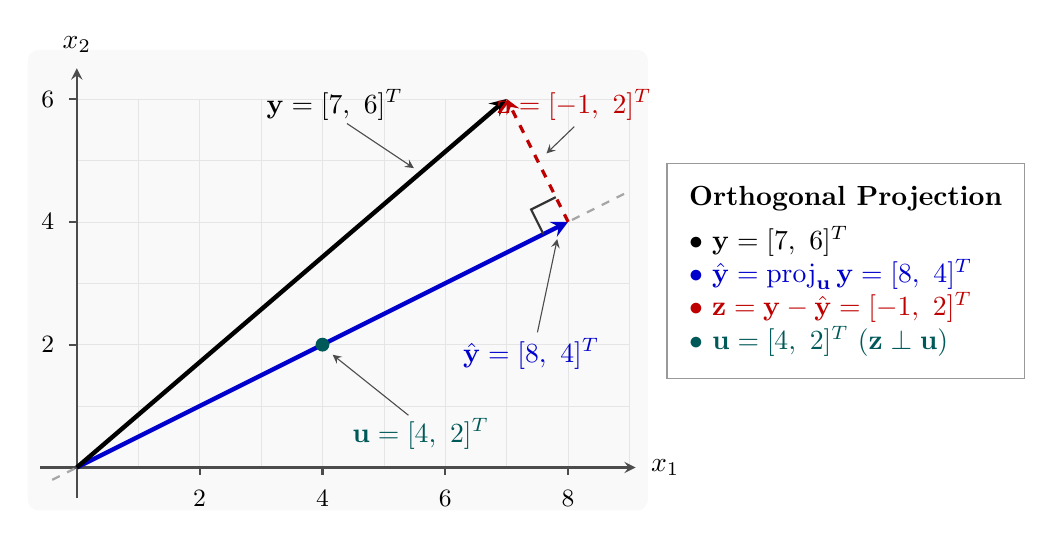
\begin{tikzpicture}[scale=0.78]
    % Layer 1: Background fill
    \fill[gray!5, rounded corners=4pt] (-0.8, -0.7) rectangle (9.3, 6.8);

    % Layer 2: Grid lines, coordinate axes, and tick marks
    \draw[step=1, gray!20, very thin] (0, 0) grid (9, 6);
    \draw[->, >=stealth, thick, black!70] (-0.6, 0) -- (9.1, 0);
    \draw[->, >=stealth, thick, black!70] (0, -0.5) -- (0, 6.5);
    \foreach \x in {2, 4, 6, 8} {
        \draw[thick, black!70] (\x, 0) -- (\x, -0.12);
    }
    \foreach \y in {2, 4, 6} {
        \draw[thick, black!70] (0, \y) -- (-0.12, \y);
    }

    % Layer 3: Primary plots, vectors, and geometric markers
    \draw[dashed, gray!70, thick] (-0.4, -0.2) -- (9.0, 4.5);
    \draw[->, >=stealth, ultra thick, blue!80!black] (0, 0) -- (8, 4);
    \draw[->, >=stealth, ultra thick, black] (0, 0) -- (7, 6);
    \draw[->, >=stealth, very thick, dashed, red!75!black] (8, 4) -- (7, 6);
    \draw[thick, black!80] (7.598, 3.799) -- (7.397, 4.201) -- (7.799, 4.402);
    \fill[teal!70!black] (4, 2) circle (3.2pt);

    % Layer 4: Axis labels, callouts, and single-node legend
    \node[right=2pt, black] at (9.1, 0) {$x_1$};
    \node[above=2pt, black] at (0, 6.5) {$x_2$};
    \foreach \x in {2, 4, 6, 8} {
        \node[below=2pt, black] at (\x, -0.12) {\small $\x$};
    }
    \foreach \y in {2, 4, 6} {
        \node[left=2pt, black] at (-0.12, \y) {\small $\y$};
    }

    \draw[->, >=stealth, shorten >=3pt, black!70] (4.4, 5.6) -- (5.6, 4.8);
    \node[black] at (4.2, 5.9) {$\displaystyle \mathbf{y} = [7,\ 6]^T$};

    \draw[->, >=stealth, shorten >=3pt, black!70] (5.4, 0.85) -- (4.06, 1.92);
    \node[teal!70!black] at (5.6, 0.55) {$\displaystyle \mathbf{u} = [4,\ 2]^T$};

    \draw[->, >=stealth, shorten >=3pt, black!70] (7.5, 2.2) -- (7.85, 3.85);
    \node[blue!80!black] at (7.4, 1.85) {$\displaystyle \hat{\mathbf{y}} = [8,\ 4]^T$};

    \draw[->, >=stealth, shorten >=3pt, black!70] (8.1, 5.55) -- (7.55, 5.02);
    \node[red!75!black] at (8.1, 5.9) {$\displaystyle \mathbf{z} = [-1,\ 2]^T$};

    \node[anchor=west, align=left, draw=black!40, fill=white, inner sep=8pt, text=black] at (9.6, 3.2) {
        \textbf{Orthogonal Projection}\\[4pt]
        \textcolor{black}{$\bullet\ \mathbf{y} = [7,\ 6]^T$} \\
        \textcolor{blue!80!black}{$\bullet\ \hat{\mathbf{y}} = \operatorname{proj}_{\mathbf{u}}\mathbf{y} = [8,\ 4]^T$} \\
        \textcolor{red!75!black}{$\bullet\ \mathbf{z} = \mathbf{y} - \hat{\mathbf{y}} = [-1,\ 2]^T$} \\
        \textcolor{teal!70!black}{$\bullet\ \mathbf{u} = [4,\ 2]^T\ (\mathbf{z} \perp \mathbf{u})$}
    };
\end{tikzpicture}
\end{center}

\textbf{Final Answer:} (a) $\hat{\mathbf{y}} = \begin{bmatrix} 8 \\ 4 \end{bmatrix}$, (b) $\mathbf{z} = \begin{bmatrix} -1 \\ 2 \end{bmatrix}$ ($\mathbf{z} \cdot \mathbf{u} = 0$), (c) Both sides equal $85$.

\medskip
\textbf{Problem 14 (Original Statement):} Let $\mathbf{y} = \begin{bmatrix} 1 \\ 3 \\ 5 \end{bmatrix}$ and $L = \operatorname{Span}\{\mathbf{u}\} \subset \mathbb{R}^3$, where $\mathbf{u} = \begin{bmatrix} 1 \\ -1 \\ 2 \end{bmatrix}$. (a) Decompose $\mathbf{y} = \hat{\mathbf{y}} + \mathbf{z}$ with $\hat{\mathbf{y}} \in L$ and $\mathbf{z} \perp L$. (b) Find the shortest distance from $\mathbf{y}$ to $L$.

\textbf{Solution:}
\begin{enumerate}[label=(\alph*)]
    \item Compute $\mathbf{y} \cdot \mathbf{u} = (1)(1) + (3)(-1) + (5)(2) = 1 - 3 + 10 = 8$ and $\mathbf{u} \cdot \mathbf{u} = 1^2 + (-1)^2 + 2^2 = 6$. The component of $\mathbf{y}$ in $L$ is:
    \[
    \hat{\mathbf{y}} = \operatorname{proj}_{\mathbf{u}}\mathbf{y} = \frac{8}{6}\begin{bmatrix} 1 \\ -1 \\ 2 \end{bmatrix} = \frac{4}{3}\begin{bmatrix} 1 \\ -1 \\ 2 \end{bmatrix} = \begin{bmatrix} 4/3 \\ -4/3 \\ 8/3 \end{bmatrix}
    \]
    The orthogonal component is:
    \[
    \mathbf{z} = \mathbf{y} - \hat{\mathbf{y}} = \begin{bmatrix} 1 \\ 3 \\ 5 \end{bmatrix} - \begin{bmatrix} 4/3 \\ -4/3 \\ 8/3 \end{bmatrix} = \begin{bmatrix} -1/3 \\ 13/3 \\ 7/3 \end{bmatrix}
    \]
    Check $\mathbf{z} \perp L$: $\mathbf{z} \cdot \mathbf{u} = \left(-\frac{1}{3}\right)(1) + \left(\frac{13}{3}\right)(-1) + \left(\frac{7}{3}\right)(2) = \frac{-1 - 13 + 14}{3} = 0$, so $\mathbf{z}$ is orthogonal to every scalar multiple of $\mathbf{u}$ in $L$.
    \item The point on $L$ closest to $\mathbf{y}$ is $\hat{\mathbf{y}}$, so the shortest distance is $\|\mathbf{y} - \hat{\mathbf{y}}\| = \|\mathbf{z}\|$:
    \[
    \|\mathbf{z}\| = \frac{1}{3}\sqrt{(-1)^2 + 13^2 + 7^2} = \frac{1}{3}\sqrt{1 + 169 + 49} = \frac{\sqrt{219}}{3}
    \]
\end{enumerate}
\textbf{Final Answer:} (a) $\mathbf{y} = \begin{bmatrix} 4/3 \\ -4/3 \\ 8/3 \end{bmatrix} + \begin{bmatrix} -1/3 \\ 13/3 \\ 7/3 \end{bmatrix}$; (b) $\frac{\sqrt{219}}{3}$.

\medskip
\textbf{Problem 15 (Original Statement):} Let $\mathbf{u}, \mathbf{y} \in \mathbb{R}^n$ with $\mathbf{u} \neq \mathbf{0}$. (a) Prove $\operatorname{proj}_{c\mathbf{u}}\mathbf{y} = \operatorname{proj}_{\mathbf{u}}\mathbf{y}$ for $c \neq 0$. (b) Prove $\operatorname{proj}_{\mathbf{u}}(\operatorname{proj}_{\mathbf{u}}\mathbf{y}) = \operatorname{proj}_{\mathbf{u}}\mathbf{y}$. (c) Compute $\operatorname{proj}_{\mathbf{u}}\mathbf{y}$ efficiently for $\mathbf{u} = \begin{bmatrix} 1/5 \\ -2/5 \\ 2/5 \end{bmatrix}$ and $\mathbf{y} = \begin{bmatrix} 4 \\ 1 \\ 8 \end{bmatrix}$.

\textbf{Solution:}
\begin{enumerate}[label=(\alph*)]
    \item Using homogeneity and bilinearity of the inner product for any $c \in \mathbb{R} \setminus \{0\}$:
    \[
    \operatorname{proj}_{c\mathbf{u}}\mathbf{y} = \frac{\mathbf{y} \cdot (c\mathbf{u})}{(c\mathbf{u}) \cdot (c\mathbf{u})}(c\mathbf{u}) = \frac{c(\mathbf{y} \cdot \mathbf{u})}{c^2(\mathbf{u} \cdot \mathbf{u})}(c\mathbf{u}) = \frac{c^2}{c^2}\left(\frac{\mathbf{y} \cdot \mathbf{u}}{\mathbf{u} \cdot \mathbf{u}}\right)\mathbf{u} = \operatorname{proj}_{\mathbf{u}}\mathbf{y}
    \]
    \item Let $\alpha = \frac{\mathbf{y} \cdot \mathbf{u}}{\mathbf{u} \cdot \mathbf{u}} \in \mathbb{R}$, so $\operatorname{proj}_{\mathbf{u}}\mathbf{y} = \alpha\mathbf{u}$. Applying $\operatorname{proj}_{\mathbf{u}}$ again:
    \[
    \operatorname{proj}_{\mathbf{u}}(\alpha\mathbf{u}) = \frac{(\alpha\mathbf{u}) \cdot \mathbf{u}}{\mathbf{u} \cdot \mathbf{u}}\mathbf{u} = \alpha\left(\frac{\mathbf{u} \cdot \mathbf{u}}{\mathbf{u} \cdot \mathbf{u}}\right)\mathbf{u} = \alpha\mathbf{u} = \operatorname{proj}_{\mathbf{u}}\mathbf{y}
    \]
    \item Scale $\mathbf{u}$ by $c = 5$ to obtain $\mathbf{v} = 5\mathbf{u} = \begin{bmatrix} 1 \\ -2 \\ 2 \end{bmatrix}$. By part (a), $\operatorname{proj}_{\mathbf{u}}\mathbf{y} = \operatorname{proj}_{\mathbf{v}}\mathbf{y}$:
    \[
    \mathbf{y} \cdot \mathbf{v} = (4)(1) + (1)(-2) + (8)(2) = 4 - 2 + 16 = 18, \qquad \mathbf{v} \cdot \mathbf{v} = 1^2 + (-2)^2 + 2^2 = 9
    \]
    Therefore:
    \[
    \operatorname{proj}_{\mathbf{u}}\mathbf{y} = \frac{18}{9}\begin{bmatrix} 1 \\ -2 \\ 2 \end{bmatrix} = 2\begin{bmatrix} 1 \\ -2 \\ 2 \end{bmatrix} = \begin{bmatrix} 2 \\ -4 \\ 4 \end{bmatrix}
    \]
\end{enumerate}
\textbf{Final Answer:} (a) and (b) proved above; (c) $\operatorname{proj}_{\mathbf{u}}\mathbf{y} = \begin{bmatrix} 2 \\ -4 \\ 4 \end{bmatrix}$.

\medskip
\textbf{Problem 16 (Original Statement):} Let $\mathbf{u} = \begin{bmatrix} 2 \\ -1 \\ 2 \end{bmatrix}$ and $\mathbf{y} = \begin{bmatrix} a \\ 4 \\ b \end{bmatrix}$ in $\mathbb{R}^3$. Suppose $\operatorname{proj}_{\mathbf{u}}\mathbf{y} = \begin{bmatrix} 4 \\ -2 \\ 4 \end{bmatrix}$ and $\|\mathbf{y}\|^2 = 77$. (a) Find the linear equation relating $a$ and $b$. (b) Find all possible vectors $\mathbf{y}$.

\textbf{Solution:}
\begin{enumerate}[label=(\alph*)]
    \item Notice that $\operatorname{proj}_{\mathbf{u}}\mathbf{y} = \begin{bmatrix} 4 \\ -2 \\ 4 \end{bmatrix} = 2\mathbf{u}$. Comparing with the projection formula $\left(\frac{\mathbf{y} \cdot \mathbf{u}}{\mathbf{u} \cdot \mathbf{u}}\right)\mathbf{u}$ and using $\mathbf{u} \cdot \mathbf{u} = 2^2 + (-1)^2 + 2^2 = 9$, we obtain:
    \[
    \frac{\mathbf{y} \cdot \mathbf{u}}{9} = 2 \implies \mathbf{y} \cdot \mathbf{u} = 18
    \]
    Evaluating $\mathbf{y} \cdot \mathbf{u} = 2a + (4)(-1) + 2b = 2a + 2b - 4$ gives:
    \[
    2a + 2b - 4 = 18 \implies 2a + 2b = 22 \implies a + b = 11
    \]
    \item From $\|\mathbf{y}\|^2 = 77$, we have $a^2 + 4^2 + b^2 = 77 \implies a^2 + b^2 = 61$. Substitute $b = 11 - a$:
    \[
    a^2 + (11 - a)^2 = 61 \implies 2a^2 - 22a + 121 = 61 \implies 2a^2 - 22a + 60 = 0
    \]
    Divide by $2$ and factor:
    \[
    a^2 - 11a + 30 = 0 \implies (a - 5)(a - 6) = 0
    \]
    If $a = 5$, then $b = 6$; if $a = 6$, then $b = 5$. Both satisfy $2a - 4 + 2b = 18$ and $a^2 + 16 + b^2 = 77$.
\end{enumerate}
\textbf{Final Answer:} (a) $a + b = 11$; (b) $\mathbf{y} = \begin{bmatrix} 5 \\ 4 \\ 6 \end{bmatrix}$ or $\mathbf{y} = \begin{bmatrix} 6 \\ 4 \\ 5 \end{bmatrix}$.

\subsection{Orthogonal Complements and Fundamental Subspaces}

\textbf{Problem 17 (Original Statement):} Let $W = \operatorname{Span}\{\mathbf{v}_1, \mathbf{v}_2\} \subset \mathbb{R}^4$, where $\mathbf{v}_1 = \begin{bmatrix} 1 \\ -2 \\ 3 \\ 1 \end{bmatrix}$ and $\mathbf{v}_2 = \begin{bmatrix} 2 \\ 1 \\ 0 \\ -1 \end{bmatrix}$. (a) Check if $\mathbf{x} = \begin{bmatrix} 1 \\ 1 \\ 1 \\ -2 \end{bmatrix} \in W^{\perp}$. (b) Check if $\mathbf{z} = \begin{bmatrix} 1 \\ 0 \\ -1 \\ 2 \end{bmatrix} \in W^{\perp}$. (c) Explain why checking $\mathbf{z} \cdot \mathbf{v}_1 = 0$ and $\mathbf{z} \cdot \mathbf{v}_2 = 0$ suffices for all $\mathbf{w} \in W$.

\textbf{Solution:}
\begin{enumerate}[label=(\alph*)]
    \item Compute dot products with the spanning vectors:
    \[
    \mathbf{x} \cdot \mathbf{v}_1 = 1(1) + 1(-2) + 1(3) + (-2)(1) = 1 - 2 + 3 - 2 = 0
    \]
    \[
    \mathbf{x} \cdot \mathbf{v}_2 = 1(2) + 1(1) + 1(0) + (-2)(-1) = 2 + 1 + 0 + 2 = 5 \neq 0
    \]
    Because $\mathbf{x}$ is not orthogonal to $\mathbf{v}_2 \in W$, $\mathbf{x} \notin W^{\perp}$.
    \item Compute dot products for $\mathbf{z}$:
    \[
    \mathbf{z} \cdot \mathbf{v}_1 = 1(1) + 0(-2) + (-1)(3) + 2(1) = 1 + 0 - 3 + 2 = 0
    \]
    \[
    \mathbf{z} \cdot \mathbf{v}_2 = 1(2) + 0(1) + (-1)(0) + 2(-1) = 2 + 0 + 0 - 2 = 0
    \]
    Since $\mathbf{z}$ is orthogonal to every spanning vector of $W$, $\mathbf{z} \in W^{\perp}$.
    \item Every vector $\mathbf{w} \in W$ is a linear combination $\mathbf{w} = c_1\mathbf{v}_1 + c_2\mathbf{v}_2$ for some $c_1, c_2 \in \mathbb{R}$. By distributivity of the inner product:
    \[
    \mathbf{z} \cdot \mathbf{w} = c_1(\mathbf{z} \cdot \mathbf{v}_1) + c_2(\mathbf{z} \cdot \mathbf{v}_2) = c_1(0) + c_2(0) = 0
    \]
    Hence $\mathbf{z}$ is orthogonal to every vector in $W$.
\end{enumerate}
\textbf{Final Answer:} (a) $\mathbf{x} \notin W^{\perp}$; (b) $\mathbf{z} \in W^{\perp}$; (c) By linearity of the inner product over spanning combinations.

\medskip
\textbf{Problem 18 (Original Statement):} Let $W = \operatorname{Span}\left\{\begin{bmatrix} 1 \\ 2 \\ -1 \\ 3 \end{bmatrix}, \begin{bmatrix} 2 \\ 5 \\ 0 \\ 4 \end{bmatrix}\right\} \subset \mathbb{R}^4$. (a) Construct $A$ with $W = \operatorname{Row}(A)$ and explain why $W^{\perp} = \operatorname{Nul}(A)$. (b) Find a basis for $W^{\perp}$. (c) Verify directly that each basis vector is orthogonal to both spanning vectors of $W$.

\textbf{Solution:}
\begin{enumerate}[label=(\alph*)]
    \item Place the transposes of the spanning vectors as the rows of $A$:
    \[
    A = \begin{bmatrix} 1 & 2 & -1 & 3 \\ 2 & 5 & 0 & 4 \end{bmatrix}
    \]
    Then $\operatorname{Row}(A) = W$. For any $\mathbf{x} \in \mathbb{R}^4$, the $i$-th entry of $A\mathbf{x}$ is the dot product of row $i$ of $A$ with $\mathbf{x}$. Thus $\mathbf{x} \in \operatorname{Nul}(A) \iff A\mathbf{x} = \mathbf{0} \iff \mathbf{x}$ is orthogonal to both spanning rows of $W \iff \mathbf{x} \in W^{\perp}$.
    \item Row-reduce $A$ to reduced echelon form:
    \[
    \begin{bmatrix} 1 & 2 & -1 & 3 \\ 2 & 5 & 0 & 4 \end{bmatrix}
    \xrightarrow{R_2 \leftarrow R_2 - 2R_1}
    \begin{bmatrix} 1 & 2 & -1 & 3 \\ 0 & 1 & 2 & -2 \end{bmatrix}
    \xrightarrow{R_1 \leftarrow R_1 - 2R_2}
    \begin{bmatrix} 1 & 0 & -5 & 7 \\ 0 & 1 & 2 & -2 \end{bmatrix}
    \]
    The solution set of $A\mathbf{x} = \mathbf{0}$ satisfies $x_1 = 5x_3 - 7x_4$ and $x_2 = -2x_3 + 2x_4$, with $x_3, x_4$ free:
    \[
    \mathbf{x} = x_3 \begin{bmatrix} 5 \\ -2 \\ 1 \\ 0 \end{bmatrix} + x_4 \begin{bmatrix} -7 \\ 2 \\ 0 \\ 1 \end{bmatrix}
    \]
    Therefore, a basis for $W^{\perp} = \operatorname{Nul}(A)$ is $\left\{ \mathbf{b}_1, \mathbf{b}_2 \right\} = \left\{ \begin{bmatrix} 5 \\ -2 \\ 1 \\ 0 \end{bmatrix}, \begin{bmatrix} -7 \\ 2 \\ 0 \\ 1 \end{bmatrix} \right\}$.
    \item Verify orthogonality with $\mathbf{r}_1 = [1,\ 2,\ -1,\ 3]^T$ and $\mathbf{r}_2 = [2,\ 5,\ 0,\ 4]^T$:
    \begin{align*}
    \mathbf{b}_1 \cdot \mathbf{r}_1 &= 5(1) + (-2)(2) + 1(-1) + 0(3) = 5 - 4 - 1 + 0 = 0, \\
    \mathbf{b}_1 \cdot \mathbf{r}_2 &= 5(2) + (-2)(5) + 1(0) + 0(4) = 10 - 10 + 0 + 0 = 0, \\
    \mathbf{b}_2 \cdot \mathbf{r}_1 &= (-7)(1) + 2(2) + 0(-1) + 1(3) = -7 + 4 + 0 + 3 = 0, \\
    \mathbf{b}_2 \cdot \mathbf{r}_2 &= (-7)(2) + 2(5) + 0(0) + 1(4) = -14 + 10 + 0 + 4 = 0.
    \end{align*}
\end{enumerate}
\textbf{Final Answer:} (a) $A = \begin{bmatrix} 1 & 2 & -1 & 3 \\ 2 & 5 & 0 & 4 \end{bmatrix}$; (b) Basis: $\left\{ \begin{bmatrix} 5 \\ -2 \\ 1 \\ 0 \end{bmatrix}, \begin{bmatrix} -7 \\ 2 \\ 0 \\ 1 \end{bmatrix} \right\}$; (c) All four inner products equal $0$.

\medskip
\textbf{Problem 19 (Original Statement):} Let $A = \begin{bmatrix} 1 & -2 \\ 2 & -3 \\ -1 & 1 \end{bmatrix}$. (a) Prove $(\operatorname{Col} M)^{\perp} = \operatorname{Nul}(M^T)$ for any $m \times n$ matrix $M$. (b) Find a basis for $(\operatorname{Col} A)^{\perp}$. (c) Verify whether $\mathbf{b} = \begin{bmatrix} -2 \\ 2 \\ 2 \end{bmatrix} \in (\operatorname{Col} A)^{\perp}$, and explain what this implies about the consistency of $A\mathbf{x} = \mathbf{b}$.

\textbf{Solution:}
\begin{enumerate}[label=(\alph*)]
    \item Let $\mathbf{m}_1, \dots, \mathbf{m}_n \in \mathbb{R}^m$ be the columns of $M$. Since these columns span $\operatorname{Col} M$, a vector $\mathbf{y} \in \mathbb{R}^m$ belongs to $(\operatorname{Col} M)^{\perp}$ if and only if $\mathbf{m}_j \cdot \mathbf{y} = \mathbf{m}_j^T \mathbf{y} = 0$ for all $j = 1, \dots, n$. Since the rows of $M^T$ are precisely $\mathbf{m}_1^T, \dots, \mathbf{m}_n^T$, this holds if and only if $M^T \mathbf{y} = \mathbf{0}$, i.e., $\mathbf{y} \in \operatorname{Nul}(M^T)$.
    \item Compute $A^T$ and row-reduce:
    \[
    A^T = \begin{bmatrix} 1 & 2 & -1 \\ -2 & -3 & 1 \end{bmatrix}
    \xrightarrow{R_2 \leftarrow R_2 + 2R_1}
    \begin{bmatrix} 1 & 2 & -1 \\ 0 & 1 & -1 \end{bmatrix}
    \xrightarrow{R_1 \leftarrow R_1 - 2R_2}
    \begin{bmatrix} 1 & 0 & 1 \\ 0 & 1 & -1 \end{bmatrix}
    \]
    Thus $y_1 = -y_3$ and $y_2 = y_3$, with $y_3$ free. A basis for $(\operatorname{Col} A)^{\perp} = \operatorname{Nul}(A^T)$ is $\left\{ \begin{bmatrix} -1 \\ 1 \\ 1 \end{bmatrix} \right\}$.
    \item Check $A^T \mathbf{b}$:
    \[
    A^T \mathbf{b} = \begin{bmatrix} 1 & 2 & -1 \\ -2 & -3 & 1 \end{bmatrix} \begin{bmatrix} -2 \\ 2 \\ 2 \end{bmatrix} = \begin{bmatrix} -2 + 4 - 2 \\ 4 - 6 + 2 \end{bmatrix} = \begin{bmatrix} 0 \\ 0 \end{bmatrix}
    \]
    So $\mathbf{b} \in (\operatorname{Col} A)^{\perp}$. Because $\mathbf{b} \neq \mathbf{0}$ and $\operatorname{Col} A \cap (\operatorname{Col} A)^{\perp} = \{\mathbf{0}\}$, it follows that $\mathbf{b} \notin \operatorname{Col} A$; hence the linear system $A\mathbf{x} = \mathbf{b}$ is \textbf{inconsistent} (it has no exact solution).
\end{enumerate}
\textbf{Final Answer:} (a) Proved above; (b) $\left\{ \begin{bmatrix} -1 \\ 1 \\ 1 \end{bmatrix} \right\}$; (c) $\mathbf{b} \in (\operatorname{Col} A)^{\perp}$, which implies $A\mathbf{x} = \mathbf{b}$ is inconsistent.

\subsection{Cauchy-Schwarz and Triangle Inequalities}

\textbf{Problem 20 (Original Statement):} (a) Verify $|\mathbf{u} \cdot \mathbf{v}| \le \|\mathbf{u}\|\|\mathbf{v}\|$ for $\mathbf{u} = \begin{bmatrix} 2 \\ -3 \\ 6 \end{bmatrix}$ and $\mathbf{v} = \begin{bmatrix} -4 \\ 1 \\ 2 \end{bmatrix}$. (b) Show equality holds for $\mathbf{p} = \begin{bmatrix} 3 \\ -4 \end{bmatrix}$ and $\mathbf{q} = \begin{bmatrix} -6 \\ 8 \end{bmatrix}$, and state the general equality condition.

\textbf{Solution:}
\begin{enumerate}[label=(\alph*)]
    \item Compute $\mathbf{u} \cdot \mathbf{v} = (2)(-4) + (-3)(1) + (6)(2) = -8 - 3 + 12 = 1$, so $|\mathbf{u} \cdot \mathbf{v}| = 1$. Compute the norms:
    \[
    \|\mathbf{u}\| = \sqrt{2^2 + (-3)^2 + 6^2} = \sqrt{4 + 9 + 36} = \sqrt{49} = 7, \qquad \|\mathbf{v}\| = \sqrt{(-4)^2 + 1^2 + 2^2} = \sqrt{16 + 1 + 4} = \sqrt{21}
    \]
    Thus $\|\mathbf{u}\|\|\mathbf{v}\| = 7\sqrt{21} \approx 32.08$. Since $1 \le 7\sqrt{21}$, the Cauchy-Schwarz Inequality holds.
    \item Compute $\mathbf{p} \cdot \mathbf{q} = (3)(-6) + (-4)(8) = -18 - 32 = -50$, so $|\mathbf{p} \cdot \mathbf{q}| = 50$. Meanwhile:
    \[
    \|\mathbf{p}\| = \sqrt{3^2 + (-4)^2} = 5, \qquad \|\mathbf{q}\| = \sqrt{(-6)^2 + 8^2} = 10 \implies \|\mathbf{p}\|\|\mathbf{q}\| = 50
    \]
    Hence $|\mathbf{p} \cdot \mathbf{q}| = \|\mathbf{p}\|\|\mathbf{q}\|$. In general, equality holds in the Cauchy-Schwarz Inequality if and only if $\mathbf{u}$ and $\mathbf{v}$ are \textbf{linearly dependent} (i.e., one vector is a scalar multiple of the other, or at least one is $\mathbf{0}$).
\end{enumerate}
\textbf{Final Answer:} (a) $1 \le 7\sqrt{21}$; (b) Both sides equal $50$; equality holds iff $\mathbf{u}$ and $\mathbf{v}$ are linearly dependent.

\medskip
\textbf{Problem 21 (Original Statement):} Suppose $\mathbf{u}, \mathbf{v} \in \mathbb{R}^5$ satisfy $\|\mathbf{u}\| = 4$ and $\|\mathbf{v}\| = 7$. (a) Find the minimum and maximum of $\mathbf{u} \cdot \mathbf{v}$. (b) Find the minimum and maximum of $\|\mathbf{u} + \mathbf{v}\|$ and $\|\mathbf{u} - \mathbf{v}\|$. (c) Describe the orientation when $\|\mathbf{u} - \mathbf{v}\|$ is maximized.

\textbf{Solution:}
\begin{enumerate}[label=(\alph*)]
    \item By the Cauchy-Schwarz Inequality:
    \[
    |\mathbf{u} \cdot \mathbf{v}| \le \|\mathbf{u}\|\|\mathbf{v}\| = (4)(7) = 28 \implies -28 \le \mathbf{u} \cdot \mathbf{v} \le 28
    \]
    Both bounds are achievable in $\mathbb{R}^5$ by choosing $\mathbf{v} = \pm \frac{7}{4}\mathbf{u}$. Hence the minimum is $-28$ and the maximum is $28$.
    \item Expand $\|\mathbf{u} + \mathbf{v}\|^2 = \|\mathbf{u}\|^2 + 2(\mathbf{u} \cdot \mathbf{v}) + \|\mathbf{v}\|^2 = 16 + 2(\mathbf{u} \cdot \mathbf{v}) + 49 = 65 + 2(\mathbf{u} \cdot \mathbf{v})$. Using $-28 \le \mathbf{u} \cdot \mathbf{v} \le 28$:
    \[
    65 + 2(-28) \le \|\mathbf{u} + \mathbf{v}\|^2 \le 65 + 2(28) \implies 9 \le \|\mathbf{u} + \mathbf{v}\|^2 \le 121 \implies 3 \le \|\mathbf{u} + \mathbf{v}\| \le 11
    \]
    Similarly, $\|\mathbf{u} - \mathbf{v}\|^2 = 65 - 2(\mathbf{u} \cdot \mathbf{v})$, which satisfies the same bounds:
    \[
    9 \le \|\mathbf{u} - \mathbf{v}\|^2 \le 121 \implies 3 \le \|\mathbf{u} - \mathbf{v}\| \le 11
    \]
    \item $\|\mathbf{u} - \mathbf{v}\|$ achieves its maximum value of $11$ when $\mathbf{u} \cdot \mathbf{v} = -28 = -\|\mathbf{u}\|\|\mathbf{v}\|$, meaning $\cos\theta = -1$ ($\theta = \pi$); geometrically, $\mathbf{u}$ and $\mathbf{v}$ point in \textbf{strictly opposite directions}.
\end{enumerate}
\textbf{Final Answer:} (a) Min $-28$, Max $28$; (b) Min $3$, Max $11$ for both $\|\mathbf{u}+\mathbf{v}\|$ and $\|\mathbf{u}-\mathbf{v}\|$; (c) Strictly opposite directions ($\theta = \pi$).

\medskip
\textbf{Problem 22 (Original Statement):} (a) Assuming Cauchy-Schwarz, prove the Triangle Inequality $\|\mathbf{u} + \mathbf{v}\| \le \|\mathbf{u}\| + \|\mathbf{v}\|$. (b) Prove $\left(\sum_{i=1}^{n} x_i\right)^2 \le n \sum_{i=1}^{n} x_i^2$ for all real $x_1, \dots, x_n$.

\textbf{Solution:}
\begin{enumerate}[label=(\alph*)]
    \item Expand the squared norm using inner product properties, then apply $\mathbf{u} \cdot \mathbf{v} \le |\mathbf{u} \cdot \mathbf{v}| \le \|\mathbf{u}\|\|\mathbf{v}\|$:
    \begin{align*}
    \|\mathbf{u} + \mathbf{v}\|^2 &= (\mathbf{u} + \mathbf{v}) \cdot (\mathbf{u} + \mathbf{v}) \\
    &= \|\mathbf{u}\|^2 + 2(\mathbf{u} \cdot \mathbf{v}) + \|\mathbf{v}\|^2 \\
    &\le \|\mathbf{u}\|^2 + 2|\mathbf{u} \cdot \mathbf{v}| + \|\mathbf{v}\|^2 \\
    &\le \|\mathbf{u}\|^2 + 2\|\mathbf{u}\|\|\mathbf{v}\| + \|\mathbf{v}\|^2 \\
    &= \left(\|\mathbf{u}\| + \|\mathbf{v}\|\right)^2.
    \end{align*}
    Because norms are non-negative, taking square roots of both sides preserves the inequality and yields $\|\mathbf{u} + \mathbf{v}\| \le \|\mathbf{u}\| + \|\mathbf{v}\|$.
    \item Define the vectors $\mathbf{x} = \begin{bmatrix} x_1 \\ x_2 \\ \vdots \\ x_n \end{bmatrix}$ and $\mathbf{1} = \begin{bmatrix} 1 \\ 1 \\ \vdots \\ 1 \end{bmatrix}$ in $\mathbb{R}^n$. Observe that:
    \[
    \mathbf{x} \cdot \mathbf{1} = \sum_{i=1}^{n} x_i, \qquad \|\mathbf{x}\|^2 = \sum_{i=1}^{n} x_i^2, \qquad \|\mathbf{1}\|^2 = \sum_{i=1}^{n} 1^2 = n
    \]
    Squaring the Cauchy-Schwarz Inequality $|\mathbf{x} \cdot \mathbf{1}| \le \|\mathbf{x}\|\|\mathbf{1}\|$ yields $(\mathbf{x} \cdot \mathbf{1})^2 \le \|\mathbf{x}\|^2 \|\mathbf{1}\|^2$, which gives:
    \[
    \left(\sum_{i=1}^{n} x_i\right)^2 \le n \sum_{i=1}^{n} x_i^2
    \]
\end{enumerate}
\textbf{Final Answer:} Both inequalities are proved rigorously above.

\subsection{Algebraic Proofs and Geometric Identities}

\textbf{Problem 23 (Original Statement):} (a) Prove the Polarization Identity $\mathbf{u} \cdot \mathbf{v} = \frac{1}{4}\left(\|\mathbf{u} + \mathbf{v}\|^2 - \|\mathbf{u} - \mathbf{v}\|^2\right)$. (b) Compute $\mathbf{u} \cdot \mathbf{v}$ when $\|\mathbf{u} + \mathbf{v}\| = 9$ and $\|\mathbf{u} - \mathbf{v}\| = 5$.

\textbf{Solution:}
\begin{enumerate}[label=(\alph*)]
    \item Expand both squared norms using bilinearity and commutativity ($\mathbf{v} \cdot \mathbf{u} = \mathbf{u} \cdot \mathbf{v}$):
    \begin{align*}
    \|\mathbf{u} + \mathbf{v}\|^2 &= (\mathbf{u} + \mathbf{v}) \cdot (\mathbf{u} + \mathbf{v}) = \|\mathbf{u}\|^2 + 2(\mathbf{u} \cdot \mathbf{v}) + \|\mathbf{v}\|^2, \\
    \|\mathbf{u} - \mathbf{v}\|^2 &= (\mathbf{u} - \mathbf{v}) \cdot (\mathbf{u} - \mathbf{v}) = \|\mathbf{u}\|^2 - 2(\mathbf{u} \cdot \mathbf{v}) + \|\mathbf{v}\|^2.
    \end{align*}
    Subtracting the second equation from the first cancels $\|\mathbf{u}\|^2$ and $\|\mathbf{v}\|^2$:
    \[
    \|\mathbf{u} + \mathbf{v}\|^2 - \|\mathbf{u} - \mathbf{v}\|^2 = 4(\mathbf{u} \cdot \mathbf{v})
    \]
    Dividing both sides by $4$ yields $\mathbf{u} \cdot \mathbf{v} = \frac{1}{4}\left(\|\mathbf{u} + \mathbf{v}\|^2 - \|\mathbf{u} - \mathbf{v}\|^2\right)$.
    \item Substitute $\|\mathbf{u} + \mathbf{v}\| = 9$ and $\|\mathbf{u} - \mathbf{v}\| = 5$:
    \[
    \mathbf{u} \cdot \mathbf{v} = \frac{1}{4}\left(9^2 - 5^2\right) = \frac{1}{4}(81 - 25) = \frac{56}{4} = 14
    \]
\end{enumerate}
\textbf{Final Answer:} (a) Proved above; (b) $\mathbf{u} \cdot \mathbf{v} = 14$.

\medskip
\textbf{Problem 24 (Original Statement):} (a) Prove $\|a\mathbf{u} + b\mathbf{v}\|^2 + \|b\mathbf{u} - a\mathbf{v}\|^2 = (a^2 + b^2)(\|\mathbf{u}\|^2 + \|\mathbf{v}\|^2)$, and explain how $a=b=1$ gives the Parallelogram Law. (b) Prove $\|\mathbf{u} + \mathbf{v}\| = \|\mathbf{u} - \mathbf{v}\| \iff \mathbf{u} \perp \mathbf{v}$.

\textbf{Solution:}
\begin{enumerate}[label=(\alph*)]
    \item Expand each term using inner product properties:
    \begin{align*}
    \|a\mathbf{u} + b\mathbf{v}\|^2 &= (a\mathbf{u} + b\mathbf{v}) \cdot (a\mathbf{u} + b\mathbf{v}) = a^2\|\mathbf{u}\|^2 + 2ab(\mathbf{u} \cdot \mathbf{v}) + b^2\|\mathbf{v}\|^2, \\
    \|b\mathbf{u} - a\mathbf{v}\|^2 &= (b\mathbf{u} - a\mathbf{v}) \cdot (b\mathbf{u} - a\mathbf{v}) = b^2\|\mathbf{u}\|^2 - 2ab(\mathbf{u} \cdot \mathbf{v}) + a^2\|\mathbf{v}\|^2.
    \end{align*}
    Adding the two expansions cancels the cross terms $\pm 2ab(\mathbf{u} \cdot \mathbf{v})$:
    \[
    \|a\mathbf{u} + b\mathbf{v}\|^2 + \|b\mathbf{u} - a\mathbf{v}\|^2 = (a^2 + b^2)\|\mathbf{u}\|^2 + (a^2 + b^2)\|\mathbf{v}\|^2 = (a^2 + b^2)\left(\|\mathbf{u}\|^2 + \|\mathbf{v}\|^2\right)
    \]
    Setting $a = b = 1$ gives $\|\mathbf{u} + \mathbf{v}\|^2 + \|\mathbf{u} - \mathbf{v}\|^2 = 2\|\mathbf{u}\|^2 + 2\|\mathbf{v}\|^2$, which is the Parallelogram Law (the sum of the squared diagonals equals the sum of the squares of all four sides).
    \item Since vector norms are non-negative, we have a chain of equivalences:
    \begin{align*}
    \|\mathbf{u} + \mathbf{v}\| = \|\mathbf{u} - \mathbf{v}\| &\iff \|\mathbf{u} + \mathbf{v}\|^2 = \|\mathbf{u} - \mathbf{v}\|^2 \\
    &\iff \|\mathbf{u}\|^2 + 2(\mathbf{u} \cdot \mathbf{v}) + \|\mathbf{v}\|^2 = \|\mathbf{u}\|^2 - 2(\mathbf{u} \cdot \mathbf{v}) + \|\mathbf{v}\|^2 \\
    &\iff 4(\mathbf{u} \cdot \mathbf{v}) = 0 \\
    &\iff \mathbf{u} \cdot \mathbf{v} = 0 \iff \mathbf{u} \perp \mathbf{v}.
    \end{align*}
\end{enumerate}

\begin{center}
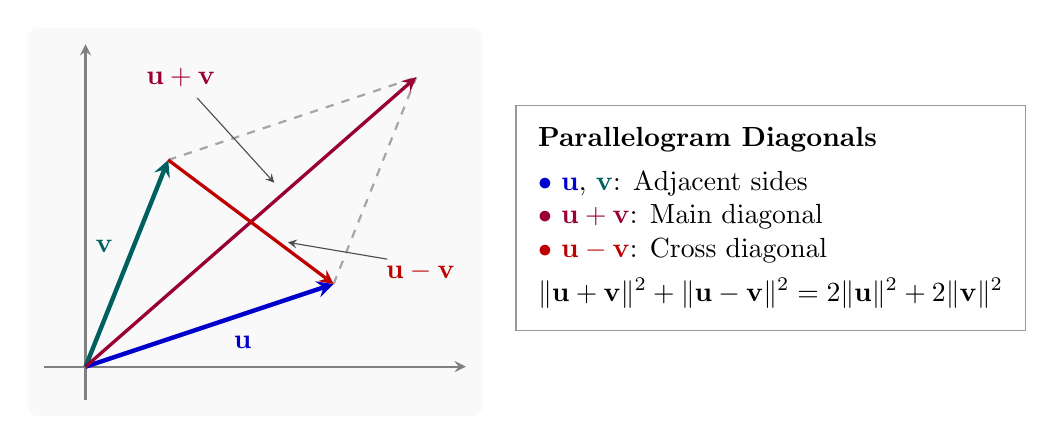
\begin{tikzpicture}[scale=1.05]
    % Layer 1: Background fill
    \fill[gray!5, rounded corners=4pt] (-0.7, -0.6) rectangle (4.8, 4.1);

    % Layer 2: Coordinate axes
    \draw[->, >=stealth, thick, black!50] (-0.5, 0) -- (4.6, 0);
    \draw[->, >=stealth, thick, black!50] (0, -0.4) -- (0, 3.9);

    % Layer 3: Parallelogram sides and diagonals
    \draw[dashed, gray!70, thick] (3, 1) -- (4, 3.5);
    \draw[dashed, gray!70, thick] (1, 2.5) -- (4, 3.5);
    \draw[->, >=stealth, ultra thick, blue!80!black] (0, 0) -- (3, 1);
    \draw[->, >=stealth, ultra thick, teal!75!black] (0, 0) -- (1, 2.5);
    \draw[->, >=stealth, very thick, purple!80!black] (0, 0) -- (4, 3.5);
    \draw[->, >=stealth, very thick, red!75!black] (1, 2.5) -- (3, 1);

    % Layer 4: Labels, callouts, and single-node legend
    \node[blue!80!black] at (1.9, 0.30) {$\mathbf{u}$};
    \node[teal!75!black, left=3pt] at (0.55, 1.45) {$\mathbf{v}$};

    \draw[->, >=stealth, shorten >=3pt, black!70] (1.35, 3.25) -- (2.35, 2.15);
    \node[purple!80!black] at (1.15, 3.5) {$\mathbf{u} + \mathbf{v}$};

    \draw[->, >=stealth, shorten >=3pt, black!70] (3.65, 1.3) -- (2.35, 1.52);
    \node[red!75!black] at (4.05, 1.15) {$\mathbf{u} - \mathbf{v}$};

    \node[anchor=west, align=left, draw=black!40, fill=white, inner sep=8pt, text=black] at (5.2, 1.8) {
        \textbf{Parallelogram Diagonals}\\[4pt]
        \textcolor{blue!80!black}{$\bullet\ \mathbf{u}$}, \textcolor{teal!75!black}{$\mathbf{v}$}: Adjacent sides \\
        \textcolor{purple!80!black}{$\bullet\ \mathbf{u} + \mathbf{v}$}: Main diagonal \\
        \textcolor{red!75!black}{$\bullet\ \mathbf{u} - \mathbf{v}$}: Cross diagonal \\[4pt]
        $\displaystyle \|\mathbf{u}+\mathbf{v}\|^2 + \|\mathbf{u}-\mathbf{v}\|^2 = 2\|\mathbf{u}\|^2 + 2\|\mathbf{v}\|^2$
    };
\end{tikzpicture}
\end{center}

\textbf{Final Answer:} Both identities and equivalences are proved above.

\medskip
\textbf{Problem 25 (Original Statement):} Let $W$ be any nonempty subset of $\mathbb{R}^n$, and define $W^{\perp} = \{\mathbf{x} \in \mathbb{R}^n \mid \mathbf{x} \cdot \mathbf{w} = 0 \text{ for all } \mathbf{w} \in W\}$. (a) If $\mathbf{y}$ is orthogonal to $\mathbf{u}$ and $\mathbf{v}$, show $\mathbf{y} \perp (c_1\mathbf{u} + c_2\mathbf{v})$. (b) Prove $W^{\perp}$ is a subspace of $\mathbb{R}^n$.

\textbf{Solution:}
\begin{enumerate}[label=(\alph*)]
    \item Given $\mathbf{y} \cdot \mathbf{u} = 0$ and $\mathbf{y} \cdot \mathbf{v} = 0$, use linearity of the dot product:
    \[
    \mathbf{y} \cdot (c_1\mathbf{u} + c_2\mathbf{v}) = c_1(\mathbf{y} \cdot \mathbf{u}) + c_2(\mathbf{y} \cdot \mathbf{v}) = c_1(0) + c_2(0) = 0
    \]
    Hence $\mathbf{y}$ is orthogonal to $c_1\mathbf{u} + c_2\mathbf{v}$.
    \item Verify the three subspace axioms for $W^{\perp} \subseteq \mathbb{R}^n$:
    \begin{enumerate}[label=\arabic*.]
        \item \textit{Zero vector:} For every $\mathbf{w} \in W$, $\mathbf{0} \cdot \mathbf{w} = 0$. Therefore $\mathbf{0} \in W^{\perp}$.
        \item \textit{Closure under addition:} Let $\mathbf{x}, \mathbf{y} \in W^{\perp}$. For any $\mathbf{w} \in W$, $(\mathbf{x} + \mathbf{y}) \cdot \mathbf{w} = \mathbf{x} \cdot \mathbf{w} + \mathbf{y} \cdot \mathbf{w} = 0 + 0 = 0$. Hence $\mathbf{x} + \mathbf{y} \in W^{\perp}$.
        \item \textit{Closure under scalar multiplication:} Let $\mathbf{x} \in W^{\perp}$ and $c \in \mathbb{R}$. For any $\mathbf{w} \in W$, $(c\mathbf{x}) \cdot \mathbf{w} = c(\mathbf{x} \cdot \mathbf{w}) = c(0) = 0$. Hence $c\mathbf{x} \in W^{\perp}$.
    \end{enumerate}
    Because all three axioms hold, $W^{\perp}$ is a subspace of $\mathbb{R}^n$.
\end{enumerate}
\textbf{Final Answer:} Linearity and all three subspace axioms are verified above.

\medskip
\textbf{Problem 26 (Original Statement):} (a) Prove $\|\mathbf{u}\| = \|\mathbf{v}\| \iff (\mathbf{u} + \mathbf{v}) \perp (\mathbf{u} - \mathbf{v})$. (b) Suppose $\mathbf{u} \cdot \mathbf{v} = \|\mathbf{u}\|^2$; prove $\mathbf{u} \perp (\mathbf{v} - \mathbf{u})$ and interpret geometrically when $\mathbf{u} \neq \mathbf{0}$.

\textbf{Solution:}
\begin{enumerate}[label=(\alph*)]
    \item Compute the inner product of the diagonals using distributivity and commutativity:
    \[
    (\mathbf{u} + \mathbf{v}) \cdot (\mathbf{u} - \mathbf{v}) = \mathbf{u} \cdot \mathbf{u} - \mathbf{u} \cdot \mathbf{v} + \mathbf{v} \cdot \mathbf{u} - \mathbf{v} \cdot \mathbf{v} = \|\mathbf{u}\|^2 - \|\mathbf{v}\|^2
    \]
    Since vector lengths are non-negative:
    \[
    (\mathbf{u} + \mathbf{v}) \perp (\mathbf{u} - \mathbf{v}) \iff \|\mathbf{u}\|^2 - \|\mathbf{v}\|^2 = 0 \iff \|\mathbf{u}\|^2 = \|\mathbf{v}\|^2 \iff \|\mathbf{u}\| = \|\mathbf{v}\|
    \]
    \item Compute $\mathbf{u} \cdot (\mathbf{v} - \mathbf{u})$ using distributivity:
    \[
    \mathbf{u} \cdot (\mathbf{v} - \mathbf{u}) = \mathbf{u} \cdot \mathbf{v} - \mathbf{u} \cdot \mathbf{u} = \mathbf{u} \cdot \mathbf{v} - \|\mathbf{u}\|^2 = \|\mathbf{u}\|^2 - \|\mathbf{u}\|^2 = 0
    \]
    Thus $\mathbf{u} \perp (\mathbf{v} - \mathbf{u})$. Geometrically, when $\mathbf{u} \neq \mathbf{0}$, $\operatorname{proj}_{\mathbf{u}}\mathbf{v} = \left(\frac{\mathbf{v} \cdot \mathbf{u}}{\mathbf{u} \cdot \mathbf{u}}\right)\mathbf{u} = \left(\frac{\|\mathbf{u}\|^2}{\|\mathbf{u}\|^2}\right)\mathbf{u} = \mathbf{u}$, meaning $\mathbf{u}$ itself is the orthogonal projection of $\mathbf{v}$ onto $\operatorname{Span}\{\mathbf{u}\}$ (the triangle with sides $\mathbf{u}$, $\mathbf{v} - \mathbf{u}$, and hypotenuse $\mathbf{v}$ has a right angle at the tip of $\mathbf{u}$).
\end{enumerate}
\textbf{Final Answer:} Both proofs and the orthogonal projection interpretation are established above.

\subsection{Conceptual Diagnostics and Pitfall Analysis}

\textbf{Problem 27 (Original Statement):} Determine whether each statement is \textbf{True} or \textbf{False}, providing a proof or counterexample: (a) $\|c\mathbf{v}\| = c\|\mathbf{v}\|$; (b) $\mathbf{u} \cdot \mathbf{v} = \mathbf{u} \cdot \mathbf{w},\ \mathbf{u} \neq \mathbf{0} \implies \mathbf{v} = \mathbf{w}$; (c) $\mathbf{0}$ is the unique vector in $W \cap W^{\perp}$; (d) $\|\mathbf{u} - \mathbf{v}\|^2 = \|\mathbf{u}\|^2 - \|\mathbf{v}\|^2$; (e) $(\mathbf{u} \cdot \mathbf{v}) \cdot \mathbf{w}$ is a well-defined scalar; (f) $\mathbf{x}$ orthogonal to a spanning set of $W \implies \mathbf{x} \in W^{\perp}$.

\textbf{Solution:}
\begin{enumerate}[label=(\alph*)]
    \item \textbf{False.} The correct scaling property is $\|c\mathbf{v}\| = |c|\|\mathbf{v}\|$. Counterexample: let $c = -2$ and $\mathbf{v} = \begin{bmatrix} 1 \\ 0 \end{bmatrix}$. Then $\|c\mathbf{v}\| = \|[-2,\ 0]^T\| = 2$, whereas $c\|\mathbf{v}\| = -2(1) = -2$.
    \item \textbf{False.} There is no cancellation law for the inner product; $\mathbf{u} \cdot (\mathbf{v} - \mathbf{w}) = 0$ only implies $\mathbf{v} - \mathbf{w} \perp \mathbf{u}$. Counterexample: let $\mathbf{u} = \begin{bmatrix} 1 \\ 0 \end{bmatrix}$, $\mathbf{v} = \begin{bmatrix} 2 \\ 1 \end{bmatrix}$, and $\mathbf{w} = \begin{bmatrix} 2 \\ -5 \end{bmatrix}$. Then $\mathbf{u} \cdot \mathbf{v} = 2 = \mathbf{u} \cdot \mathbf{w}$, yet $\mathbf{v} \neq \mathbf{w}$.
    \item \textbf{True.} Because $W$ and $W^{\perp}$ are subspaces, $\mathbf{0} \in W \cap W^{\perp}$. Conversely, if any $\mathbf{x} \in W \cap W^{\perp}$, then $\mathbf{x}$ is orthogonal to itself, so $\|\mathbf{x}\|^2 = \mathbf{x} \cdot \mathbf{x} = 0 \implies \mathbf{x} = \mathbf{0}$.
    \item \textbf{False.} The correct expansion is $\|\mathbf{u} - \mathbf{v}\|^2 = \|\mathbf{u}\|^2 - 2(\mathbf{u} \cdot \mathbf{v}) + \|\mathbf{v}\|^2$. Counterexample: let $\mathbf{u} = \begin{bmatrix} 1 \\ 0 \end{bmatrix}$ and $\mathbf{v} = \begin{bmatrix} 0 \\ 1 \end{bmatrix}$. Then $\|\mathbf{u} - \mathbf{v}\|^2 = \|[1,\ -1]^T\|^2 = 2$, whereas $\|\mathbf{u}\|^2 - \|\mathbf{v}\|^2 = 1 - 1 = 0$.
    \item \textbf{False.} The dot product $\mathbf{u} \cdot \mathbf{v}$ returns a \emph{scalar}, not a vector, so taking the dot product of the scalar $(\mathbf{u} \cdot \mathbf{v})$ with the vector $\mathbf{w}$ is mathematically undefined.
    \item \textbf{True.} Every $\mathbf{w} \in W$ has the form $\mathbf{w} = \sum_{j=1}^{p} c_j \mathbf{v}_j$. By linearity, $\mathbf{x} \cdot \mathbf{w} = \sum_{j=1}^{p} c_j (\mathbf{x} \cdot \mathbf{v}_j) = 0$, so $\mathbf{x} \in W^{\perp}$.
\end{enumerate}
\textbf{Final Answer:} (a) False, (b) False, (c) True, (d) False, (e) False, (f) True.

\medskip
\textbf{Problem 28 (Original Statement):} Identify the flaw, explain in one sentence why it is invalid, and give the correct final answer for each of parts (a)--(e).

\textbf{Solution:}
\begin{enumerate}[label=(\alph*)]
    \item \textbf{Flaw:} The student evaluated $(-5)^2$ as $-25$ instead of $+25$. \textit{Explanation:} The square of any nonzero real number is strictly positive because $(-a)^2 = (-a)(-a) = a^2$. \textbf{Correct Answer:} $\|\mathbf{v}\| = \sqrt{25 + 144} = \sqrt{169} = 13$.
    \item \textbf{Flaw:} The student computed the difference of the individual norms $|\|\mathbf{u}\| - \|\mathbf{v}\||$ instead of the norm of the difference vector $\|\mathbf{u} - \mathbf{v}\|$. \textit{Explanation:} Distance measures the length of the displacement vector connecting two points, which equals $|\|\mathbf{u}\| - \|\mathbf{v}\||$ only when the vectors point in the exact same direction. \textbf{Correct Answer:} $\|\mathbf{u} - \mathbf{v}\| = \left\|\begin{bmatrix} 5 \\ -12 \end{bmatrix}\right\| = \sqrt{25 + 144} = 13$.
    \item \textbf{Flaw:} The student divided $\mathbf{v}$ by the squared length $\|\mathbf{v}\|^2 = 6$ instead of the actual length $\|\mathbf{v}\| = \sqrt{6}$. \textit{Explanation:} Normalizing a vector requires dividing by its norm $\|\mathbf{v}\| = \sqrt{\mathbf{v} \cdot \mathbf{v}}$, whereas dividing by $\|\mathbf{v}\|^2$ produces a vector of length $1/\|\mathbf{v}\| \neq 1$. \textbf{Correct Answer:} $\hat{\mathbf{v}} = \begin{bmatrix} 2/\sqrt{6} \\ -1/\sqrt{6} \\ 1/\sqrt{6} \end{bmatrix}$.
    \item \textbf{Flaw:} The student inferred $\theta = 0$ from $\cos\theta = 0$. \textit{Explanation:} On the interval $[0, \pi]$, $\cos\theta = 0$ corresponds to a right angle $\theta = \pi/2$ radians ($90^\circ$), whereas $\theta = 0$ corresponds to $\cos\theta = 1$. \textbf{Correct Answer:} $\theta = \frac{\pi}{2}$ radians.
    \item \textbf{Flaw:} The student treated the dot product as associative and applied the dot product between a scalar and a vector. \textit{Explanation:} Because the dot product of two vectors outputs a scalar, $(\mathbf{u} \cdot \mathbf{v}) \cdot \mathbf{w}$ is a mathematically invalid type mismatch that cannot be evaluated or regrouped. \textbf{Correct Answer:} The expression $(\mathbf{u} \cdot \mathbf{v}) \cdot \mathbf{w}$ is undefined (only scalar multiplication $(\mathbf{u} \cdot \mathbf{v})\mathbf{w} = \begin{bmatrix} 20 \\ 25 \end{bmatrix}$ is valid).
\end{enumerate}
\textbf{Final Answer:} All five diagnostic flaws, explanations, and corrected answers are provided above.

\subsection{Real-World Modeling in Machine Learning and Quantitative Finance}

\textbf{Problem 29 (Original Statement):} Consider the separating hyperplane $H = \{\mathbf{x} \in \mathbb{R}^2 \mid \mathbf{w} \cdot \mathbf{x} + b = 0\}$ with $\mathbf{w} = \begin{bmatrix} 3 \\ 4 \end{bmatrix}$ and $b = -12$. (a) Verify $\mathbf{p}_1 = \begin{bmatrix} 4 \\ 0 \end{bmatrix}$ and $\mathbf{p}_2 = \begin{bmatrix} 0 \\ 3 \end{bmatrix}$ lie on $H$ and prove $\mathbf{w} \perp (\mathbf{p}_2 - \mathbf{p}_1)$. (b) Check $y_i(\mathbf{w} \cdot \mathbf{x}_i + b) \ge 1$ for $(\mathbf{x}_1, +1) = ([3,1]^T, +1)$, $(\mathbf{x}_2, -1) = ([1,2]^T, -1)$, and $(\mathbf{x}_3, +1) = ([4,2]^T, +1)$. (c) Compute $d_i = \frac{|\mathbf{w}\cdot\mathbf{x}_i + b|}{\|\mathbf{w}\|}$, identify support vectors, and find the total margin $\frac{2}{\|\mathbf{w}\|}$.

\textbf{Solution:}
\begin{enumerate}[label=(\alph*)]
    \item Evaluate $\mathbf{w} \cdot \mathbf{x} + b$ at $\mathbf{p}_1$ and $\mathbf{p}_2$:
    \[
    \mathbf{w} \cdot \mathbf{p}_1 + b = 3(4) + 4(0) - 12 = 0, \qquad \mathbf{w} \cdot \mathbf{p}_2 + b = 3(0) + 4(3) - 12 = 0
    \]
    Both points lie on $H$. Their direction vector is $\mathbf{p}_2 - \mathbf{p}_1 = \begin{bmatrix} -4 \\ 3 \end{bmatrix}$, and:
    \[
    \mathbf{w} \cdot (\mathbf{p}_2 - \mathbf{p}_1) = (3)(-4) + (4)(3) = -12 + 12 = 0
    \]
    Hence $\mathbf{w} \perp (\mathbf{p}_2 - \mathbf{p}_1)$, confirming $\mathbf{w}$ is normal to $H$.
    \item Evaluate $y_i(\mathbf{w} \cdot \mathbf{x}_i + b)$ for each labeled training example:
    \begin{align*}
    y_1(\mathbf{w} \cdot \mathbf{x}_1 + b) &= (+1)\big(3(3) + 4(1) - 12\big) = (+1)(1) = 1 \ge 1, \\
    y_2(\mathbf{w} \cdot \mathbf{x}_2 + b) &= (-1)\big(3(1) + 4(2) - 12\big) = (-1)(-1) = 1 \ge 1, \\
    y_3(\mathbf{w} \cdot \mathbf{x}_3 + b) &= (+1)\big(3(4) + 4(2) - 12\big) = (+1)(8) = 8 \ge 1.
    \end{align*}
    All three points satisfy the functional margin constraint.
    \item First compute $\|\mathbf{w}\| = \sqrt{3^2 + 4^2} = 5$. The exact geometric distances to $H$ are:
    \[
    d_1 = \frac{|1|}{5} = \frac{1}{5} = 0.2, \qquad d_2 = \frac{|-1|}{5} = \frac{1}{5} = 0.2, \qquad d_3 = \frac{|8|}{5} = \frac{8}{5} = 1.6
    \]
    Because equality holds in the functional margin constraint for $\mathbf{x}_1$ and $\mathbf{x}_2$ (both lie at minimum distance $\frac{1}{\|\mathbf{w}\|} = \frac{1}{5}$ from $H$), $\mathbf{x}_1$ and $\mathbf{x}_2$ are the \textbf{support vectors}. The total margin width separating the two classes is $\frac{2}{\|\mathbf{w}\|} = \frac{2}{5} = 0.4$.
\end{enumerate}

\begin{center}
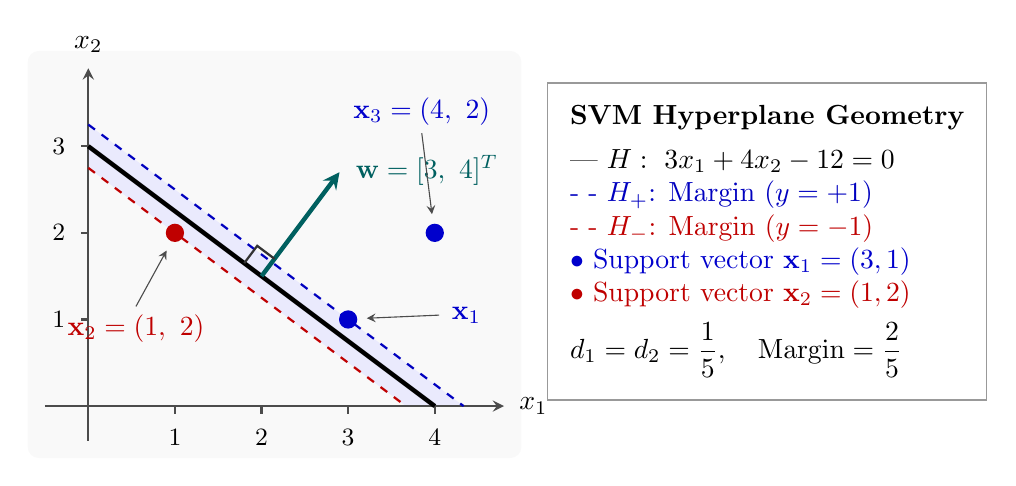
\begin{tikzpicture}[scale=1.1]
    % Layer 1: Background fill and margin strip
    \fill[gray!5, rounded corners=4pt] (-0.7, -0.6) rectangle (5.0, 4.1);
    \fill[blue!10, opacity=0.75] (0, 2.75) -- (0, 3.25) -- (4.333, 0) -- (3.667, 0) -- cycle;

    % Layer 2: Coordinate axes and tick marks
    \draw[->, >=stealth, thick, black!70] (-0.5, 0) -- (4.8, 0);
    \draw[->, >=stealth, thick, black!70] (0, -0.4) -- (0, 3.9);
    \foreach \x in {1, 2, 3, 4} {
        \draw[thick, black!70] (\x, 0) -- (\x, -0.09);
    }
    \foreach \y in {1, 2, 3} {
        \draw[thick, black!70] (0, \y) -- (-0.09, \y);
    }

    % Layer 3: Hyperplane, margin lines, normal vector, right angle, and points
    \draw[ultra thick, black] (0, 3) -- (4, 0);
    \draw[thick, dashed, blue!75!black] (0, 3.25) -- (4.333, 0);
    \draw[thick, dashed, red!75!black] (0, 2.75) -- (3.667, 0);
    \draw[->, >=stealth, ultra thick, teal!75!black] (2, 1.5) -- (2.9, 2.7);
    \draw[thick, black!80] (1.8, 1.65) -- (1.95, 1.85) -- (2.15, 1.70);

    \fill[blue!80!black] (3, 1) circle (3pt);
    \fill[blue!80!black] (4, 2) circle (3pt);
    \fill[red!75!black] (1, 2) circle (3pt);

    % Layer 4: Axis labels, callout arrows, and single-node legend
    \node[right=2pt, black] at (4.8, 0) {$x_1$};
    \node[above=2pt, black] at (0, 3.9) {$x_2$};
    \foreach \x in {1, 2, 3, 4} {
        \node[below=2pt, black] at (\x, -0.09) {\small $\x$};
    }
    \foreach \y in {1, 2, 3} {
        \node[left=2pt, black] at (-0.09, \y) {\small $\y$};
    }

    \node[teal!75!black, right=3pt] at (2.88, 2.72) {$\mathbf{w} = [3,\ 4]^T$};

    \draw[->, >=stealth, shorten >=3pt, black!70] (3.85, 3.15) -- (3.98, 2.12);
    \node[blue!80!black] at (3.85, 3.4) {$\mathbf{x}_3 = (4,\ 2)$};

    \draw[->, >=stealth, shorten >=3pt, black!70] (4.05, 1.05) -- (3.12, 1.01);
    \node[blue!80!black, right=2pt] at (4.02, 1.05) {$\mathbf{x}_1$};

    \draw[->, >=stealth, shorten >=3pt, black!70] (0.55, 1.15) -- (0.95, 1.88);
    \node[red!75!black] at (0.55, 0.9) {$\mathbf{x}_2 = (1,\ 2)$};

    \node[anchor=west, align=left, draw=black!40, fill=white, inner sep=8pt, text=black] at (5.3, 1.9) {
        \textbf{SVM Hyperplane Geometry}\\[4pt]
        \textcolor{black}{--- $H:\ 3x_1 + 4x_2 - 12 = 0$} \\
        \textcolor{blue!75!black}{- - $H_+$: Margin ($y=+1$)} \\
        \textcolor{red!75!black}{- - $H_-$: Margin ($y=-1$)} \\
        \textcolor{blue!80!black}{$\bullet$ Support vector $\mathbf{x}_1=(3,1)$} \\
        \textcolor{red!75!black}{$\bullet$ Support vector $\mathbf{x}_2=(1,2)$} \\[4pt]
        $\displaystyle d_1 = d_2 = \frac{1}{5},\quad \text{Margin} = \frac{2}{5}$
    };
\end{tikzpicture}
\end{center}

\textbf{Final Answer:} (a) $\mathbf{w} \cdot (\mathbf{p}_2 - \mathbf{p}_1) = 0$; (b) Functional margins are $1$, $1$, and $8$; (c) $d_1 = d_2 = 1/5$, $d_3 = 8/5$; support vectors are $\mathbf{x}_1, \mathbf{x}_2$; total margin is $2/5$.

\medskip
\textbf{Problem 30 (Original Statement):} Let $\mathbf{f}_1 = \begin{bmatrix} 1 \\ 1 \\ 1 \\ 1 \end{bmatrix}$, $\mathbf{f}_2 = \begin{bmatrix} 1 \\ -1 \\ 1 \\ -1 \end{bmatrix}$, and $\mathbf{p} = \begin{bmatrix} 5 \\ 1 \\ 3 \\ -1 \end{bmatrix}$ in $\mathbb{R}^4$. (a) Verify $\mathbf{f}_1 \perp \mathbf{f}_2$ and normalize both. (b) Compute $\hat{\mathbf{p}} = \operatorname{proj}_{\mathbf{f}_1}\mathbf{p} + \operatorname{proj}_{\mathbf{f}_2}\mathbf{p}$. (c) Compute $\mathbf{p}_{\perp} = \mathbf{p} - \hat{\mathbf{p}}$, verify $\mathbf{p}_{\perp} \in F^{\perp}$ for $F = \operatorname{Span}\{\mathbf{f}_1, \mathbf{f}_2\}$, and find $\frac{\|\hat{\mathbf{p}}\|^2}{\|\mathbf{p}\|^2}$.

\textbf{Solution:}
\begin{enumerate}[label=(\alph*)]
    \item Compute $\mathbf{f}_1 \cdot \mathbf{f}_2 = (1)(1) + (1)(-1) + (1)(1) + (1)(-1) = 0$, confirming the factors are orthogonal. Next, $\|\mathbf{f}_1\| = \sqrt{1+1+1+1} = 2$ and $\|\mathbf{f}_2\| = \sqrt{1+1+1+1} = 2$, so the unit risk factors are:
    \[
    \hat{\mathbf{f}}_1 = \frac{1}{2}\begin{bmatrix} 1 \\ 1 \\ 1 \\ 1 \end{bmatrix} = \begin{bmatrix} 1/2 \\ 1/2 \\ 1/2 \\ 1/2 \end{bmatrix}, \qquad \hat{\mathbf{f}}_2 = \frac{1}{2}\begin{bmatrix} 1 \\ -1 \\ 1 \\ -1 \end{bmatrix} = \begin{bmatrix} 1/2 \\ -1/2 \\ 1/2 \\ -1/2 \end{bmatrix}
    \]
    \item Compute each orthogonal projection individually ($\mathbf{f}_1 \cdot \mathbf{f}_1 = \mathbf{f}_2 \cdot \mathbf{f}_2 = 4$):
    \[
    \mathbf{p} \cdot \mathbf{f}_1 = 5 + 1 + 3 - 1 = 8 \implies \operatorname{proj}_{\mathbf{f}_1}\mathbf{p} = \frac{8}{4}\begin{bmatrix} 1 \\ 1 \\ 1 \\ 1 \end{bmatrix} = \begin{bmatrix} 2 \\ 2 \\ 2 \\ 2 \end{bmatrix}
    \]
    \[
    \mathbf{p} \cdot \mathbf{f}_2 = 5 - 1 + 3 + 1 = 8 \implies \operatorname{proj}_{\mathbf{f}_2}\mathbf{p} = \frac{8}{4}\begin{bmatrix} 1 \\ -1 \\ 1 \\ -1 \end{bmatrix} = \begin{bmatrix} 2 \\ -2 \\ 2 \\ -2 \end{bmatrix}
    \]
    Adding the two factor components gives the systematic portfolio projection:
    \[
    \hat{\mathbf{p}} = \begin{bmatrix} 2 \\ 2 \\ 2 \\ 2 \end{bmatrix} + \begin{bmatrix} 2 \\ -2 \\ 2 \\ -2 \end{bmatrix} = \begin{bmatrix} 4 \\ 0 \\ 4 \\ 0 \end{bmatrix}
    \]
    \item Compute the idiosyncratic residual portfolio:
    \[
    \mathbf{p}_{\perp} = \mathbf{p} - \hat{\mathbf{p}} = \begin{bmatrix} 5 \\ 1 \\ 3 \\ -1 \end{bmatrix} - \begin{bmatrix} 4 \\ 0 \\ 4 \\ 0 \end{bmatrix} = \begin{bmatrix} 1 \\ 1 \\ -1 \\ -1 \end{bmatrix}
    \]
    Verify orthogonality to both spanning vectors of $F$:
    \[
    \mathbf{p}_{\perp} \cdot \mathbf{f}_1 = 1 + 1 - 1 - 1 = 0, \qquad \mathbf{p}_{\perp} \cdot \mathbf{f}_2 = 1 - 1 - 1 + 1 = 0
    \]
    Since $\mathbf{p}_{\perp}$ is orthogonal to both $\mathbf{f}_1$ and $\mathbf{f}_2$, $\mathbf{p}_{\perp} \in F^{\perp}$. Finally, compute the squared norms:
    \[
    \|\mathbf{p}\|^2 = 5^2 + 1^2 + 3^2 + (-1)^2 = 36, \qquad \|\hat{\mathbf{p}}\|^2 = 4^2 + 0^2 + 4^2 + 0^2 = 32
    \]
    (Notice $\|\mathbf{p}_{\perp}\|^2 = 1^2 + 1^2 + (-1)^2 + (-1)^2 = 4$, satisfying $\|\mathbf{p}\|^2 = \|\hat{\mathbf{p}}\|^2 + \|\mathbf{p}_{\perp}\|^2 = 32 + 4 = 36$.) The proportion of variance proxy explained by the factor subspace is:
    \[
    \frac{\|\hat{\mathbf{p}}\|^2}{\|\mathbf{p}\|^2} = \frac{32}{36} = \frac{8}{9} \approx 88.89\%
    \]
\end{enumerate}
\textbf{Final Answer:} (a) $\mathbf{f}_1 \cdot \mathbf{f}_2 = 0$, $\hat{\mathbf{f}}_1 = \frac{1}{2}[1,\ 1,\ 1,\ 1]^T$, $\hat{\mathbf{f}}_2 = \frac{1}{2}[1,\ -1,\ 1,\ -1]^T$; (b) $\hat{\mathbf{p}} = [4,\ 0,\ 4,\ 0]^T$; (c) $\mathbf{p}_{\perp} = [1,\ 1,\ -1,\ -1]^T \in F^{\perp}$, proportion explained $= \frac{8}{9} \approx 88.89\%$.

\newpage
\section{End-of-Document Concept Checklist and Question Index}

For quick revision and self-assessment, Table~\ref{tab:concept-map-end} repeats the complete concept checklist and exact question mapping for this section.

\begin{center}
\renewcommand{\arraystretch}{1.5}
\begin{tabularx}{\textwidth}{p{4.6cm} >{$\displaystyle}X<{$} l}
\toprule
\textbf{Concept / Problem Type} & \multicolumn{1}{l}{\textbf{Core Formula / Key Technique}} & \textbf{Problem(s)} \\
\midrule
Inner Product and Matrix Transpose Computation & \mathbf{u} \cdot \mathbf{v} = \mathbf{u}^T \mathbf{v} = \sum_{i=1}^{n} u_i v_i & 1, 2, 13, 30 \\
\addlinespace[4pt]
Vector Norm, Negative Squares, and Scalar Pull-Out & \|\mathbf{v}\| = \sqrt{\mathbf{v} \cdot \mathbf{v}},\quad \|c\mathbf{v}\| = |c|\|\mathbf{v}\| & 3, 4, 5, 27, 28 \\
\addlinespace[4pt]
Normalization, Unit Vectors, and Integer Scaling Trick & \hat{\mathbf{u}} = \frac{1}{\|\mathbf{v}\|}\mathbf{v}\quad (\text{clear denominators first}) & 5, 6, 28, 30 \\
\addlinespace[4pt]
Distance and Angle Between Vectors & \operatorname{dist}(\mathbf{u}, \mathbf{v}) = \|\mathbf{u} - \mathbf{v}\|,\quad \cos\theta = \frac{\mathbf{u}\cdot\mathbf{v}}{\|\mathbf{u}\|\|\mathbf{v}\|} & 7, 8, 9, 28, 29 \\
\addlinespace[4pt]
Orthogonality, Parameters, and Pythagorean Theorem & \mathbf{u} \perp \mathbf{v} \iff \mathbf{u}\cdot\mathbf{v} = 0 \iff \|\mathbf{u}+\mathbf{v}\|^2 = \|\mathbf{u}\|^2 + \|\mathbf{v}\|^2 & 10, 11, 12, 30 \\
\addlinespace[4pt]
Orthogonal Projection and Line Decomposition & \operatorname{proj}_{\mathbf{u}}\mathbf{y} = \left(\frac{\mathbf{y}\cdot\mathbf{u}}{\mathbf{u}\cdot\mathbf{u}}\right)\mathbf{u},\quad \mathbf{y} = \hat{\mathbf{y}} + \mathbf{z}\ (\mathbf{z} \perp \mathbf{u}) & 13, 14, 15, 16, 26, 30 \\
\addlinespace[4pt]
Orthogonal Complements and Fundamental Subspaces & W^{\perp\vphantom{A}},\quad \operatorname{Row}(A)^{\perp\vphantom{A}} = \operatorname{Nul}(A),\quad \operatorname{Col}(A)^{\perp\vphantom{A}} = \operatorname{Nul}(A^T) & 17, 18, 19, 25, 27, 30 \\
\addlinespace[4pt]
Cauchy-Schwarz and Triangle Inequalities & |\mathbf{u}\cdot\mathbf{v}| \le \|\mathbf{u}\|\|\mathbf{v}\|,\quad \|\mathbf{u}+\mathbf{v}\| \le \|\mathbf{u}\| + \|\mathbf{v}\| & 20, 21, 22 \\
\addlinespace[4pt]
Algebraic Proofs and Geometric Vector Identities & \|\mathbf{u}+\mathbf{v}\|^2 + \|\mathbf{u}-\mathbf{v}\|^2 = 2\|\mathbf{u}\|^2 + 2\|\mathbf{v}\|^2 & 23, 24, 25, 26 \\
\addlinespace[4pt]
Conceptual Diagnostics and ``Find the Flaw'' Traps & (\mathbf{u}\cdot\mathbf{v})\mathbf{w}\ \text{vs.\ invalid}\ (\mathbf{u}\cdot\mathbf{v})\cdot\mathbf{w},\ \text{missing}\ \sqrt{\cdot} & 4, 7, 27, 28 \\
\addlinespace[4pt]
Real-World Modeling (SVM Margin and Quant Finance) & d_i = \frac{|\mathbf{w}\cdot\mathbf{x}_i + b|}{\|\mathbf{w}\|},\quad \text{margin} = \frac{2}{\|\mathbf{w}\|},\quad \text{PCA factors} & 29, 30 \\
\bottomrule
\end{tabularx}
\captionof{table}{End-of-document concept checklist and question reference index.}
\label{tab:concept-map-end}
\end{center}

\end{document}